%%%%%%%%%%%%%%%%%%%%%%%%%%%%%%%%%%%%%%%%%%%%%%%%%%%%%%%%%%%%%%%%%%%%%%%%%%%%%%%%%%%%%%%%%%%%%%%%%%%%%%%%%%%%%%%%%%%%%%%%%%%%%%%%%%%%%%%%%%%%%%%%%%%%%%%%%%%
% This is just an example/guide for you to refer to when submitting manuscripts to Frontiers, it is not mandatory to use Frontiers .cls files nor frontiers.tex  %
% This will only generate the Manuscript, the final article will be typeset by Frontiers after acceptance.   
%                                              %
%                                                                                                                                                         %
% When submitting your files, remember to upload this *tex file, the pdf generated with it, the *bib file (if bibliography is not within the *tex) and all the figures.
%%%%%%%%%%%%%%%%%%%%%%%%%%%%%%%%%%%%%%%%%%%%%%%%%%%%%%%%%%%%%%%%%%%%%%%%%%%%%%%%%%%%%%%%%%%%%%%%%%%%%%%%%%%%%%%%%%%%%%%%%%%%%%%%%%%%%%%%%%%%%%%%%%%%%%%%%%%

%%% Version 3.4 Generated 2018/06/15 %%%
%%% You will need to have the following packages installed: datetime, fmtcount, etoolbox, fcprefix, which are normally inlcuded in WinEdt. %%%
%%% In http://www.ctan.org/ you can find the packages and how to install them, if necessary. %%%
%%%  NB logo1.jpg is required in the path in order to correctly compile front page header %%%

\documentclass[utf8]{frontiersSCNS} % for Science, Engineering and Humanities and Social Sciences articles
%\documentclass[utf8]{frontiersHLTH} % for Health articles
%\documentclass[utf8]{frontiersFPHY} % for Physics and Applied Mathematics and Statistics articles

%\setcitestyle{square} % for Physics and Applied Mathematics and Statistics articles
\usepackage{url,hyperref,lineno,microtype,subcaption}
\usepackage[onehalfspacing]{setspace}

\linenumbers


% Leave a blank line between paragraphs instead of using \\


\def\keyFont{\fontsize{8}{11}\helveticabold }
\def\firstAuthorLast{Z. Cao {et~al.}} %use et al only if is more than 1 author
\def\Authors{Zhixuan Cao\,$^{1,2}$ Marcus Bursik\,$^{3}$  Qingyuan Yang\,$^{4,5}$ Abani Patra\,$^{\star,1,6}$}
% Affiliations should be keyed to the author's name with superscript numbers and be listed as follows: Laboratory, Institute, Department, Organization, City, State abbreviation (USA, Canada, Australia), and Country (without detailed address information such as city zip codes or street names).
% If one of the authors has a change of address, list the new address below the correspondence details using a superscript symbol and use the same symbol to indicate the author in the author list.
\def\Address{$^{1}$ Mechanical and Aerospace Engineering Department, SUNY Buffalo, Buffalo, NY, USA\\
$^{2}$Fluids Business Unit, ANSYS Inc, Lebanon, NH, USA \\
$^{3}$Center for Geohazards Studies, SUNY Buffalo, Buffalo, NY, USA  \\
$^{4}$Earth Observatory of Singapore,  Singapore,  Singapore\\
$^{5}$The Asian School of the Environment,  Nanyang Technological University, Singapore,  Singapore\\
$^{6}$Data Intensive Studies Center,  Tufts University, Medford, MA, USA}
% The Corresponding Author should be marked with an asterisk
% Provide the exact contact address (this time including street name and city zip code) and email of the corresponding author
\def\corrAuthor{Abani Patra}

\def\corrEmail{abani.patra@tufts.edu}

\begin{document}
\onecolumn
\firstpage{1}

\title[VATD Based on 3D Plume Model]{Simulating the transport and dispersal of volcanic ash clouds with initial conditions created by a 3D plume model} 

\author[\firstAuthorLast ]{\Authors} %This field will be automatically populated
\address{} %This field will be automatically populated
\correspondance{} %This field will be automatically populated

\extraAuth{}% If there are more than 1 corresponding author, comment this line and uncomment the next one.
%\extraAuth{corresponding Author2 \\ Laboratory X2, Institute X2, Department X2, Organization X2, Street X2, City X2 , State XX2 (only USA, Canada and Australia), Zip Code2, X2 Country X2, email2@uni2.edu}


\maketitle


\begin{abstract}

%%% Leave the Abstract empty if your article does not require one, please see the Summary Table for full details.
\section{}
VATD (volcanic ash transport and dispersion) models simulate atmospheric transport of ash starting from a source originating at the volcano represented by concentration of ash with height. Most VATD models use a source of some prescribed shape calibrated against an empirical expression for the height-mass eruption rate (MER) relation.
The actual vertical ash distribution in volcanic plumes usually varies from case to case and have complex dependencies on eruption source parameters and atmospheric conditions.
We present here for the first time the use of a 3D (three-dimensional) plume model to represent the ash cloud source without any assumption regarding plume geometry. By eliminating assumed behavior associated with a semi-empirical plume geometry, the predictive skill of VATD simulations is greatly improved.
To date, no VATD simulation adopts initial conditions created from first principles based on a 3D plume simulation. We use our recently developed volcanic plume model based on a 3D smoothed-particle hydrodynamic Lagrangian method, and couple the output to a standard Lagrangian VATD model.  We apply the coupled model to historical eruptions to illustrate the effectiveness of the approach.
Our investigation reveals that initial particle distribution in the vertical direction has more impact on transport of ash clouds than does the horizontal distribution. Comparison with satellite data indicates that ash particles are concentrated through the depth of the volcanic umbrella cloud, and much lower than observed maximum plume height.

\tiny
 \keyFont{ \section{Keywords:}VATD, volcano, 3D plume model, initial conditions, numerical simulation, SPH, Pinatubo, ash transport, ash dispersal} %All article types: you may provide up to 8 keywords; at least 5 are mandatory.
\end{abstract}

\section{Introduction}
Volcanic ash, the fine-grained fraction of tephra can be widely dispersed to synoptic and global scales, and can lead to a degradation of air quality and pose threats to aviation \citep{tupper2007facing}. Identification, tracking and modeling the future movement of volcanic ash help route and schedule flights to avoid ash clouds. Numerical estimation of ash distribution using known and forecast wind fields is necessary if we are to accurately predict ash cloud propagation and spread. Numerous VATD (volcanic ash transport and dispersion) models have been developed by both civil and military aviation, and meteorological agencies to provide forecasts of ash cloud motion \citep{witham2007comparison}. New techniques have been integrated into VATDs to satisfy increasing demands for different types of output, model accuracy and forecast reliability. This contribution explores a method for creating initial conditions for VATD simulations, which promises to improve prediction capability.

\citet{fero2009simulating} and \citet{stohl2011determination} showed that initial source conditions have significant effects on simulation of volcanic ash transport. Traditional VATD simulation requires key global descriptors of the volcanic plume, especially plume height, grain size, eruption duration and mass loading, or alternatively, a mass eruption rate (MER). No matter how these global descriptors are obtained, they are used to furnish the initial conditions for VATDs in the form of a line-source term of a spatio-temporal distribution of particle mass. It is a common practice to pick values for these global descriptors using an empirical expression for the height-MER relation. The empirical expression is written as a function of several parameters, including the key global descriptors. The values for the descriptors can also be found by parameter calibration \citep[e.g.][]{fero2008simulation,fero2009simulating, stohl2011determination, zidikheri2017estimation}. One-dimensional (1D) plume models serve as an alternative option to provide values. For example, \citet{bursik2012estimation} used the 1D model puffin \citep{bursik2001effect} to generate estimates of mass eruption rate and grain size. In some cases, an extra step is adopted to spread ash particles from the line source horizontally, resulting in an initial ash cloud in 3D space. The horizontal spreading depends on an empirical expression. For example, the VATD model Puff spreads particles from the line source uniformly in the horizontal direction within a given radius using an empirical expression generated from the output of puffin. Considering the complexities of volcanic eruptions, the actual ash distribution in the initial ash cloud should vary from case to case and with time, making it difficult to find one general expression that is suitable for all cases. It is useful therefore to investigate alternative ways for creating initial ash clouds without assumptions regarding plume geometry, or numerical inversion. This provides the major motivation of this paper.

VATD models can be categorized into Lagrangian particle tracking and Eulerian advection-diffusion types. Among several available particle tracking models \citep[e.g.][]{walko1995hypact, searcy1998puff, d1998modeling, draxler1998overview} and advection-diffusion models \citep[e.g.][]{bonadonna2005total, folch2009fall3d, schwaiger2012ash3d}, we adopt a particle tracking model, Puff \citep{tanaka1991development,searcy1998puff}, as the primary VATD model. Puff can accept a 3D point cloud description of the starting ash cloud as an initial condition, which makes it technically easier to couple with 3D plume models. Puff initializes a discrete number of tracers that represent a sample of the eruption cloud, and calculates transport, turbulent dispersion, and fallout for each representative tracer. A cylinder emanating vertically from the volcano summit to a specified maximum height is the standard approach to provide a simple model of the geometry of a typical ash column. Puff minimally requires horizontal wind field data. The ``restart'' feature of Puff makes it technically feasible to accommodate the hand-off between a plume simulation and the Puff simulation in terms of time and length scales.

We also implement one of the most widely used models for atmospheric trajectory and dispersion calculations, the Hybrid Single-Particle Lagrangian Integrated Trajectory model (HYSPLIT) \citep{stein2015noaa, rolph2017real}, developed by NOAA's Air Resources Laboratory. HYSPLIT is able to simulate phenomena from simple back trajectories, to very sophisticated computations of transport, mixing, chemical transformation, and deposition of pollutants and hazardous materials. It  is used in this study to better understand simulation results from Puff.

Besides parameter calibration, 1D plume models have been used to obtain global descriptors of volcanic plumes. 1D plume models \citep [e.g.][]{woods1988fluid, bursik2001effect, mastin2007user, de2015plume, folch2016fplume, pouget2016sensitivity} solve the equations of motion in 1D using simplifying assumptions, and hence depend on estimation of certain parameters, especially those related to the entrainment of air, which is evaluated based on two coefficients: a coefficient due to turbulence in the rising buoyant jet, and one due to the crosswind field. Different 1D models adopt different entrainment coefficients based on a specific formulation or calibration against well-documented case studies. The feedback from plume to atmosphere is usually ignored in 1D models. While these 1D models generated well-matched results with 3D models for plumes that are dominated by wind (often called weak plumes) much greater variability is observed for strong plume scenarios \citep{bursik2009volcanic, costa2016results}. On the other hand, 3D numerical models for volcanic plumes based on first principles and having few parametrized coefficients \citep{oberhuber1998volcanic, neri2003multiparticle, suzuki2005numerical, cerminara2016ashee, cao2018plume} naturally create a 3D ash cloud, which could serve directly as an initial state of the volcanic material for VATDs. However, there is no VATD simulation using such 3D ash clouds as initial conditions. In this paper, we will carry out VATD simulations using an initial state for the ash cloud based on 3D plume simulations, generated with Plume-SPH \citep{cao2018plume, cao2017data}. The implementation techniques described in this paper can be applied to any combination of VATD model and 3D plume model even though our investigation is based on a specific VATD model and plume model.

The 1991 eruption of Pinatubo volcano is used as a case study. Pinatubo erupted between June 12 and 16, 1991, after weeks of precursory activity. The climactic phase started on June 15 at 0441 UTC and ended around 1341 UTC \citep{holasek1996satellite}. The climactic phase generated voluminous pyroclastic flows, and sent Plinian and co-ignimbrite ash and gas columns to great altitudes \citep{scott1996pyroclastic}. The evolution of the Pinatubo ash and $SO_2$ clouds was tracked using visible \citep{holasek1996satellite}, ultraviolet (Total Ozone Mapping Spectrometer; TOMS) \citep{guo2004re} and infrared sensors, including the Advanced Very High-Resolution Radiometer (AVHRR) \citep{guo2004particles}. There is sufficient observational data to estimate the eruption conditions for the climactic phase of the eruption \citep{suzuki2009three}. The availability of calibrated eruption conditions and extensive observational data regarding ash cloud transport make the Pinatubo eruption an ideal case study.

\section{Materials and Methods} \label{sec:Methodology}

\subsection {Plume-SPH Model} \label{sec:plume-sph}
Plume-SPH  \citep{cao2018plume} is designed to describe an injection of well mixed solid and volcanic gas from a circular vent above a flat surface into a stratified stationary atmosphere. The basic assumptions of the model are: 
\begin{enumerate}
\item Molecular viscosity and heat conduction is neglected since turbulent energy and momentum exchange are dominant.
\item Erupted material consisting of solid with different size and mixture of gases is assumed to be well mixed and behave like a single phase fluid (phase 2) which is valid for eruptions with fine particles and ash.
\item Air,which  is assumed to be well mixed mixture of different gases,  is assumed to be another phase (phase 1).
\item Assume thermodynamic equilibrium and dynamic equilibrium between the two phases. As a result, both phases share the common energy equation and momentum equations.
\item All other microphysical processes (such as the phase changes of \texorpdfstring{H\textsubscript{2}O}, aggregation, disaggregation, absorption of gas on the surface of solids, solution of gas into a liquid) and chemical processes are not considered in this model.
\item The effect of wind, is also not yet considered in this model. 
\end{enumerate}

Based on above assumptions, the governing equations of our model are given as:
\begin{align}
\dfrac{\partial \rho}{\partial t} + \nabla \cdot \left(\rho \textbf{v}\right) = 0 \label{eq:gov-cs-rho} \\
\dfrac{\partial \rho \xi}{\partial t} + \nabla \cdot \left(\rho \xi \textbf{v}\right) = 0 \label{eq:gov-cs-ks}\\
\dfrac{\partial \rho \textbf{v}}{\partial t} + \nabla \cdot \left(\rho \textbf{v} \textbf{v} + p\textbf{I}\right) = \rho \textbf{g} \label{eq:gov-cs-v} \\
\dfrac{\partial \rho E}{\partial t} + \nabla \cdot \left[\left(\rho E + p \right)\textbf{v}\right] = \rho \textbf{g} \cdot\textbf{v} \label{eq:gov-cs-e}
\end{align}
where $\rho$ is the density, $\textbf{v}$ is the velocity, $\xi$ is the mass fraction of ejected material, $\textbf{g}$ is the gravitational acceleration, $\textbf{I}$ is a unit tensor.
$E = e + K $ is the total energy which is a summation of kinetic energy $K$ and internal energy $e$.
An additional equation is required to close the system. In this model, the equation for closing the system is the following EOS (equation of state).
\begin{equation}
p = \left(\gamma_m - 1\right)\rho e \label{eq:EOS}
\end{equation}
where
\begin{equation}
\gamma_m = R_m/C_{vm} + 1 \label{eq:gov-gm}
\end{equation}
\begin{equation}
R_m = \xi_g R_g + \xi_a R_a  \label{eq:gov-Rm}
\end{equation}
\begin{equation}
C_{vm} = \xi_s C_{vs} + \xi_g C_{vg} + \xi_a C_{va} \label{eq:gov-Cvm}
\end{equation}
\begin{equation}
\xi_a = 1 - \xi \label{eq:gov-na}
\end{equation}
\begin{equation}
\xi_g = \xi \cdot \xi_{g0} \label{eq:gov-ng}
\end{equation}
\begin{equation}
\xi_s = \xi - \xi_g \label{eq:gov-ns}
\end{equation}
where, $C_v$ is the specific heat with constant volume, $R$ is the gas constant. $\xi$ is the mass fraction of erupted material. The subscript $m$ represents mixture of ejected material and air, $s$ represents solid portion in the ejected material, $g$ represents gas portion in the ejected material, $a$ represents air, $0$ represents phyiscal properties of erupted material. $\xi_{g0}$ is the mass fraction of vapor in the erupted material.

Three different boundary conditions are applied in this model. At the vent, temperature of erupted material $T$, eruption velocity $\textbf{v}$, the mass fraction of vapor in erupted material $\xi_{g0}$ and mass discharge rate $\dot M$ are given. The pressure of erupted material $p$ is assumed to be the same as ambient pressure for pressure-balanced eruption. The radius of vent is determined from $\rho$, $\dot M$ and $\textbf{v}$.  Non-slip wall boundary condition is applied to the flat ground, where we enforce the velocity to be zero. With further assumption that the ground is adiabatic, internal energy flux, which consists of heat flux and energy flux carried by mass flux, vanishes on the wall boundary. Pressure outlet boundary condition is applied to the surrounding atmosphere where the pressure is given. Except for the pressure,  boundary values for density, velocity, and energy are determined by numerical calculation naturely. The initial condition for Plume-SPH is created based on atmosphere profile before the eruption. 

The governing equations,  EOS, boundary conditions, and initial conditions establish a complete mathematic model. The model is then discretized using smoothed particle hydrodynamics (SPH) method. The computational domain is discretized by SPH particles. The current version, Plume-SPH 1.0 \citep{cao2018plume}, uses two types of SPH particles: 1) particles of phase 1 to represent ambient air, and 2) particles of phase 2 to represent erupted material. So before the eruption, the computational domain is fully occupied by particles of phase 1. During the eruption, particles of phase 2 are injected into the computational domain. The discretized model is then converted into computational software (Plume-SPH) based on a parallel data management framework \citep{cao2017data}.

The input parameters for Plume-SPH include the eruption condition at vent, the material properties, and atmosphere profile. The eruption parameters, material properties and atmosphere for the ``Strong plume--no wind'' case in the recent comparison study on eruptive column models \citep {costa2016results} are adopted. Eruption conditions and material properties are listed in Table \ref{tab:input_parameters_plume_simulation}. Note that the density of erupted material at the vent and radius of the vent can be computed from the given parameters. The eruption pressure is assumed to be the same as the atmospheric pressure at the vent, hence is not given in the table. The vertical profiles of atmospheric properties were  based on the reanalysis data from ECMWF (European Centre for Medium-Range Weather Forecasts) for the period corresponding to the climactic phase of the Pinatubo eruption. 

\subsection{Puff and Initial Ash Cloud} \label{sec:puff-model}
 Puff \citep{tanaka1991development,searcy1998puff} is a dynamic pollutant tracer model. the model is based on a 3D Lagrangian form of the fluid mechanics, in which the material transport is represented by the fluid motion, and diffusion is parameterized by a stochastic process of random walk. Here, the model is constructed by a sufficiently large number of  Lagrangian tracer particles with a random variables $\textbf{R}_i(t) = (x(t),y(t),z(t))$, where $ i = 1 \sim M$, which represent position vectors of particles from the origin of the ash source at the time $t$. $M$ is total number of  Lagrangian tracer particles,  a sample of all the ash particles. 
\begin{linenomath*}
\begin{equation}
\textbf{R}_i(t+\Delta t) = \textbf{R}_i(t) + \textbf{W}(t)\Delta t + \textbf{Z}(t)\Delta t + \textbf{S}_i(t) \Delta t
\end{equation}
\end{linenomath*}
Here, $\textbf{W}$ accounts for wind advection, $\textbf{Z}$  is generated by Gaussian random numbers and accounts for turbulent dispersion, and $\textbf{S}$ is the terminal gravitational fallout velocity or settling speed, which depends on a tracer's size.

To start a Puff simulation, it requires a collection of tracer particles as the initial condition, which can be generated by Puff according to several parameters given by user. The tracer particles has three basic properties, age, size and position. The age of each particle is the elapsed time from when they were released from the site. Ash particles in the initial ash cloud has zero ages. Ash size distribution is initialized using a Gussian shape on a logarithmic scale. According to mean and standard deviation provided by user, Puff will assign size to each particle. Puff initialize the position of each particle according to semiempirical expressions. The height of each particle is determined according to specified distribution from the surface ($1000 mbar \cong 0 m$) to the top of the plume height, $H_{max}$, which is given by user.

The most commonly used distribution in Puff is Poisson distribution. For the Poisson distribution, the vertical height of ash particles is given by Eq. (\ref{eq:Poisson-plume-shape}):
\begin{equation}
H=H_{max} - 0.5 H_{width}*P+H_{width}R
\label{eq:Poisson-plume-shape}
\end{equation}
where $P$ is an integral value drawn from a Poisson distribution of unit mean, $R$ is a uniformly distributed random number between 0 and 1, $H_{max}$ is the maximum plume height, $H_{width}$ represents an approximate vertical range over which the ash will be distributed.
Another commonly used vertical ash distribution in VATD simulation is Suzuki. For the Suzuki plume shape \citep{suzuki1983theoretical}, the ash mass vertical distribution is assumed to follow the Eq. (Eq. (\ref{eq:Suzuki-plume-shape})):
\begin{equation}
Q(z)=Q_m* \frac{k^2(1-z/H_{max})exp\left(k(z/H_{max} -1 )\right)}{H_{max}\left[1-(1+k)exp(-k)\right]}
\label{eq:Suzuki-plume-shape}
\end{equation}
Where $Q_m$ is the total mass of erupted material, $k$ is shape factor, which is an adjustable constant that controls ash distribution with height. A low value of $k$ gives a roughly uniform distribution of mass with elevation, while high values of $k$ concentrate mass near the plume top.
For Poisson distribution, besides the plume height $H_{max}$, there is another user specified parameter, $H_{width}$, which also affect the vertical ash distribution. For Suzuki distribution, besides the plume height $H_{max}$, there is another user specified parameter, $k$, which also affect the vertical ash distribution.

Puff initialize the horizontal distribution of ash particles according to semiempirical expression as well. Puff uses a uniformly distributed random process to determine ash particle locations in a circle centered on the volcano site. The maximum radius (at plume top) at which a particle can be located is given as ``horizontal spread''. The horizontal displacement from a vertical line above the volcano is a random value within a circle of which the radius equals the ``horizontal spread'' multiplied by the ratio of the particle height $H$ to the maximum $H_{max}$. So the resulting shape of the particle distribution within the plume is an inverted cone in which particles are located directly over the volcano at the lowest level and extend out further horizontally with increasing plume height.
\begin{equation}
r(H)= r_{max} * H / H_{max} * R
\label{eq:horizontal-particle-distribution} 
\end{equation}
where $r(H)$ is the radius of the horizontal circle, whithin which, all particles at the height of $H$ locate. $r_{max}$ is the horizontal spread. $H$ is the height, $R$ is an uniformly distributed random number between 0 and 1.

In summary, given user has chosen Poisson distribution for particle distribution in the vertical direction, there are three user specified parameters that control the tracer particle distribution in the initial ash cloud: $H_{max}$, $H_{width}$, and $r_{max}$. User can optimize or calibrate these parameters to adjust the initial condition of Puff so that the simulated results match better with observations, such as satellite imagery or pilot reports. Besides the initial ash cloud,  other input parameters for Puff are diffusivity in the vertical and horizontal directions, start and end time of the eruption, and eruption duration. When creating initial conditions from output of Plume-SPH, the total number of Lagrangian tracers is the count of all SPH particles of phase 2 in the plume. The same total number of Lagrangian tracers are used when creating initial ash cloud based on semiempirical expressions. All input parameters for Puff are list in Table \ref{tab:input_parameter_Puff_simulation}.

\subsection{Creation of Initial Ash Cloud} \label{sec:create-initial-condition}
The steps to create an initial ash cloud based on the raw output of Plume-SPH are shown in Fig. \ref{fig:create-initial-ash-plume-sph}.
The method proposed consists in generating the initial ash cloud directly from Plume-SPH, foregoing assumptions and estimates, or inverse modeling, regarding ash injection height and timing.
We use Plume-SPH as an example, noting that for other 3D plume models, the steps would be similar. The initial ash cloud is created from SPH particles of phase 2, which represents the erupted material in the model.

After reaching the maximum rise height and starting to spread horizontally, particles of phase 2 form an initial umbrella cloud (Fig. \ref{fig:Plume-SPH-Pinatubo-ash-cloud}). The 3D plume simulation is considered complete once the umbrella cloud begins to form. Parcels that will be transported by the ambient wind are those above the ``corner'' region, where mean plume motion is horizontal rather than vertical.

Considering that SPH particles are only discretization points, each is assigned a grain size according to a given total grain size distribution (TGSD) \citep{paladio1996tephra}, and a concentration according to the mass and volumetric eruption rate. The Plume-SPH discretization points are thus switched to Puff Lagrangian tracer particles having grain sizes and concentrations. The coordinates of these tracer particles, which are initially in the local Cartesian coordinate system of Plume-SPH, are converted into Puff's global coordinate system, which is given in terms of $(longitude, latitude, height)$. Puff takes the initial ash cloud, consisting of the collection of Lagrangian tracer particles with grain size and concentration, and propagates from time $t$ to time $t+\Delta t$ via solution to an advection/diffusion equation.

To summarize, there are four steps to create an initial ash cloud from the raw output of Plume-SPH:
\begin{enumerate}
\item filter by SPH particle type to select SPH particles that represent erupted material (phase 2)
\item filter by a mean velocity threshold to select the upper part (above the ``corner'' region) dominated by horizontal transport
\item switch SPH discretization points to Lagrangian tracer particles, by assigning grain size to each particle
\item convert coordinates of the SPH Lagrangian tracers into the VATDs' geographic coordinate system
\end{enumerate}
The features of the volcanic plume and resulting initial ash cloud used in the case study are shown in Fig. \ref{fig:Plume-SPH-Pinatubo-ash-cloud}. It is important to point out that since both Plume-SPH and Puff are based on the Lagrangian method, there is no extra step of conversion between an Eulerian grid and Lagrangian particles.

Table \ref{tab:VATDs-source-term-determination} compares three different methods for creating initial conditions for a VATD simulation: 1) creating initial conditions based on parameter calibration without any plume model (method 1), 2) creating initial conditions based on output of a 1D plume model (method 2), 3) extracting an initial ash cloud from a 3D plume simulation (method 3). The first method determines all global descriptors of volcanic plumes based on calibration. An initial line source or ash cloud is then created according to a semiempirical plume shape expression. Both of the other two methods depend on plume models. However, 3D plume models can generate initial ash clouds in 3D space, while 1D plume models only generate global descriptors of a plume, so a semiempirical expression or transformation is still needed to create a 3D initial ash cloud. 

\subsection{Puff Restart}

The plume and ash transport models are run at different time scales and length scales. The spatial and temporal resolutions of the plume simulations are much finer than those of the ash transport model. It takes tens of minutes ($600 s$ in this case) for the Pinatubo plume to reach a steady height. However the eruption persisted for a few hours (9 hours for the climactic phase of Pinatubo eruption), and it may be necessary to track ash transport for days following an eruption. At present, it is too expensive computationally to do 3D plume simulations of several hours in real time. In order to handle the difference in time scale, we mimic a continuing eruption with intermittent pulses releasing ash particles. In particular, we restart Puff at an interval of $600 s$, i.e., the physical time of the plume simulation to reach a steady height. At every Puff restart, we integrate the output of the last Puff simulation and Plume-SPH into a new ash cloud. This new ash cloud serves as a new initial condition with which to restart a Puff simulation. A sketch demonstrating the overall restart process is shown in Fig. (\ref{fig:Restart-Puff}). The total number of Lagrangian tracer particles used in Puff thus equals the summed number of particles in all releases. The total number of tracer particles is therefore no longer a user-selected parameter.  \citet{fero2008simulation} proposed using more realistic time-dependent plume heights. We do not adopt that strategy here for simplicity, although the idea would be straightforward in execution, given time-dependent eruption conditions.

\section{Results}

Transport of volcanic ash resulting from the Pinatubo eruption on June 15, 1991, is simulated using two different initial conditions.
The first type of initial condition is created in a traditional way according to key global descriptors ($H_{max}$, $H_{width}$ and $r_{max}$) and the semiempirical plume shape expressions. We use the observed top height ($40 km$) and two other parameters assigned semiempirically \citep{bursik2012estimation}. The second type of initial condition is created by the new method proposed in this paper. To create initial conditions using the new method described in this paper, the plume rise is simulated first by Plume-SPH. Then the initial ash cloud is obtained by processing the raw output of Plume-SPH following steps described in Sec. \ref{sec:create-initial-condition}. Except for initial conditions, the simulation parameters that control the VATD simulation are the same for both simulations. Simulated ash transport results are compared against observations.

The simulation results using different initial conditions are compared with TOMS images and AVHRR BTD ash cloud map imagery (Fig. \ref{fig:Plume-SPH-Puff-ash-cloud}).  The differences between simulated ash transport by the ``Semiempirical initial cloud + Puff'' and ``Plume-SPH+ Puff'' conditions are significant. The simulated ash concentration based on the initial conditions created from Plume-SPH is qualitatively closer to observation than that based on the semiempirical plume shape expression. At 23 hours and 31 hours after the beginning of the climactic phase, the ``Plume-SPH + Puff'' simulation generates ash footprints that are  closer to observations, especially in forecasting the location where there is a high concentration of ash. However, ash just west of Pinatubo observed in satellite images does not show up in ``Plume-SPH + Puff'' simulation results. This disparity is likely due to the fact that Pinatubo continued erupting after the climactic phase, while we only simulate the climactic phase. The ``Semiempirical initial cloud + Puff'' simulation, however, forecasts an ash distribution more spatially restricted than observation. The location of the high concentration region is far northwest of observation.  Around 55 hours after the beginning of the climactic phase, the disparity between observation and simulation becomes more obvious. Ash in the ``Semiempirical initial cloud + Puff'' simulation is located too far west of the observation. The high concentration area of the ``Plume-SPH + Puff'' simulation, even though closer to observation than that of the ``Semiempirical initial cloud + Puff'' simulation, has also propagated further than observation.

Except for the initial conditions, both simulations adopt the same parameters and wind field data. That is to say, the only difference between these two simulations is the initial distribution of ash parcels. The main difference between simulation results from the ``Plume-SPH + Puff'' and the ``Semiempirical initial cloud + Puff'' runs can be directly attributed to the initial ash particle distribution, which we discuss in detail in the following section.

\subsection{Importance of Maximum Height ($H_{max}$)}

In this section, we discuss the vertical distribution of ash particles in the initial ash cloud.
The majority of volcanic ash particles are usually  injected at an elevation lower than the maximum height. For instance, \citet{holasek1996satellite, holasek1996experiments} reported the maximum Pinatubo plume height as $\sim 39 km$ while the cloud heights were estimated at $\sim 20  - 25$ km . \citet{self1993atmospheric} reported that the maximum plume height could have been $>35$ km, but that plume heights were $23 \sim 28$ km after $\sim 15-16$ hours. The neutral buoyancy height of the Pinatubo aerosol cloud was estimated with different methods at: $\sim 17-26 km$ (lidar) by \citet{defoor1992early}, $\sim 20-23$ km (balloon) by \citet{deshler1992balloonborne}, $\sim 17-28$ km (lidar) by \citet{jager1992pinatubo}, and $\sim 17-25 km$ (lidar) by \citet{avdyushin19931}. Based on comparison between simulated clouds with early infrared satellite imagery of Pinatubo, \citet{fero2008simulation} reported that the majority of ash was transported between $16$ km and $18$ km. These observations make good physical sense, as particles are concentrated near the intrusion height of the umbrella cloud, not near the plume top, because the plume top is due to momentum overshoot. However, the empirical expressions for the height-MER relation, which are commonly adopted to create initial conditions for VATD simulations, tend to place the majority of ash particles closer to the top if one uses observed maximum height in the empirical expressions.

Here we investigate two commonly used plume shapes, the Poisson and Suzuki.
Particle distributions (in terms of mass percentage or particle number percentage) in the vertical direction in the initial ash cloud are shown in Fig. \ref{fig:Particle-distribution-Plume-SPH-vs-semiempirical}. In that figure, the vertical particle distribution based on Plume-SPH output is compared with the vertical particle distribution created based on semiempirical shape expressions. Both Poisson and Suzuki distributions in Fig. \ref{fig:Particle-distribution-Plume-SPH-vs-semiempirical} take $H_{max} = 40$ km, which is close to the reported observation of maximum height. When adopting the Poisson distribution, see (c) in  Fig. \ref{fig:Particle-distribution-Plume-SPH-vs-semiempirical}, the majority of the particles are between $30 km \sim 40 km$. Obviously, the Poisson function distributes the majority of ash at a higher elevation than was observed \citep[e.g.][]{fero2008simulation}. As for the Suzuki distribution, (d) in  Fig. \ref{fig:Particle-distribution-Plume-SPH-vs-semiempirical}, the majority of ash particles also occur in a range that is significantly higher than $25 $ km. As for initial ash clouds based on Plume-SPH simulation, most ash particles are distributed between $\sim 17-  28$ km, which matches well with observations. The maximum height is also consistent with observation. To summarize, using a semiempirical plume shape expression generates an unrealistic initial ash cloud even if we use the observed maximum plume height.

For the Poisson and Suzuki distributions, the maximum in ash particles cannot be lower without changing the maximum height. To distribute the majority of ash particles at a lower elevation, the maximum height must be reduced to a value smaller than the observed maximum height. Adjusting parameters such as maximum height in the empirical expression is actually the traditional source term calibration method. A set of initial ash clouds using different maximum heights based on the Poisson distribution is shown in Fig. \ref{fig:Particle-distribution-Plume-calibrate-semiempirical}). The maximum heights adopted in plume shape expressions are not obtained from any plume model or observation of plume height, but by \textit{a posteriori} calibration to later-observed ash cloud transport heights.

The ash clouds created by the Poisson distribution with different maximum heights are used as initial conditions in Puff simulations, whose results are shown in Fig. \ref{fig:discussion-initial-ash}. Except for the maximum height, all other parameters for creating an initial ash cloud are the same as those in Table \ref{tab:input_parameter_Puff_simulation}. Of course, the range over which the majority of ash particles is located is lower when using lower maximum heights.  Figure \ref{fig:discussion-initial-ash} thus shows that the maximum height has a significant influence on the ash transport simulation. When the maximum height is $10 $ km, the high concentration area  lags behind that observed.  If the designated maximum height is $35 $ km, the high concentration area propagates faster and is more spatially confined than observed. When using a maximum height of $\sim 41000$ m, the high concentration area propagates faster and the footprint is narrower than in both observation and ``Pume-SPH + Puff'' simulation results (see Fig. \ref{fig:Plume-SPH-Puff-ash-cloud}). The simulated high concentration area is closest to ``Plume-SPH + Puff'' simulation results when assigning a maximum height of $30$ km. The low-concentration front of the volcanic ash cloud propagates faster than observed, and is located far west of the high concentration areas. A low concentration tail area also appears in the simulation results while there is no such tail in the observed imagery, although this could be the result of imagery calibration or sensitivity. Simulation results based on a calibrated maximum height of $30 $ km show a footprint similar to those of ``Plume-SPH + Puff'', although smaller in terms of area. However, the initial ash cloud created by a Poisson distribution with maximum height around $20 $ km generates the best match ash with observation. That is to say, a maximum height lower than the real maximum height is required by the Poisson plume shape to distribute ash particles at elevations comparable to the ``true'' ash distribution. Our hypothesis regarding the disparity between the ``Semiempirical initial cloud + Puff'' simulations and observation is confirmed. Since the initial condition of vertical ash distribution has such a dominant effect on VATD simulation, it is critical for the forecast capability of VATD simulations to explore more accurate and adaptive ways for establishing the initial ash distribution, especially methods that do not rely on \textit{a posteriori} parameter calibration or inversion.

\subsection{Effect of Vertical Spread ($H_{width}$)}
In the previous section, we explored the effects of adjusting the maximum height to change the vertical ash distribution at the source. In this section, we investigate the importance of another parameter in the semiempirical Poisson expression. We vary the ``vertical spread'' ($H_{width}$ in Puff) in the range $\sim 3 - 10$ km. A set of initial ash clouds  with different vertical spreads are shown in Fig. \ref{fig:Particle-distribution-Plume-calibrate-semiempirical}. Except for vertical spread, all other parameters for creating an initial ash cloud are the same as those in Table \ref{tab:input_parameter_Puff_simulation}. The vertical width of the region within which the majority of ash particles are located becomes narrower when a smaller value for the vertical spread parameter is used, but changing it has no obvious effect on the height at which the largest fraction of ash particles is injected (essentially the height of a mode in ash distribution). The ash clouds based on different vertical spread parameters are then used as initial conditions in Puff simulations.

The results are shown in Fig. \ref{fig:discussion-initial-ash}.  Adjusting of the vertical spread changes particle distribution in the vertical direction, and thus, not surprisingly affects the VATD simulation results. None of the VATD simulations based on initial ash clouds with vertical spreads equal to 3, 5 or 10 km yield better results than do VATD simulations based on initial conditions created by Plume-SPH (see Fig. \ref{fig:discussion-initial-ash}).

The calibration tests on vertical spread, carried out here, are certainly not exhaustive. One could do a more comprehensive calibration throughout the multi-dimensional parameter space (for Poisson distribution, the parameter space is two dimensional) and find better results. In addition, with a more complicated semiempirical plume shape expression, one could have more control over plume shape and might be able to get an initial condition that yields a more accurate ash transport forecast. However, more complicated and adaptable plume shape expressions imply a higher dimensional parameter space, which requires more effort in calibration, even though the degrees of freedom to adjust plume shape are still limited.  Creating initial conditions based on 3D plume simulations is more adaptive to various cases and yields results as good as or better than calibration of the poorly-constrained semi-empirical parameter, vertical spread.

\subsection{Horizontal Ash Distribution}

The differences between the semiempirical plume particle distribution and actual (or simulated by the 3D plume model) are not only in the vertical direction. The importance of the horizontal distance of each initial ash particle from a line extending upward from the volcano is investigated in this section.  Puff uses a uniformly distributed random process to determine ash particle locations in a circle centered on the volcano site as described in section \ref{sec:puff-model}. For the output of Plume-SPH, an effective (maximum) radius is determined according to a given threshold of ash concentration, following \citet {cerminara2016large}. A time averaged, spatial integration of the dynamic 3D flow field is conducted to remove significant fluctuations in time and space. Fig. \ref{fig:radius-comparison} compares radius of the initial ash clouds created by 3D plume simulations with that assumed in the semiempirical plume shape expression adopted in Puff. It is impossible for the simple, assumed plume shapes to capture the complex and more realistic shapes developed by  Plume-SPH. Additional parameterization may generate more reasonable shapes, but these would continue to be \textit{ad hoc}, none would likely to have the potential fidelity of the 3D simulation to reality, and adding a temporally changing distribution would be difficult.

Comparison between cross-sectional views of the initial ash clouds is shown in Fig. \ref{fig:initial-cloud-horizontal}. The cross-sectional view of horizontal particle distribution using the semiempirical method (last figure in Fig. \ref{fig:initial-cloud-horizontal}) is similar to a cross-sectional view of a simulated 3D plume, in a general sense. However, for simulated 3D plumes, the ash particle distribution in cross section varies with height, which factor would become increasingly important with increasing wind speed, were wind speed to be included in the estimate of initial plume shape. It is difficult for the semiempirical expressions to accommodate such a complex distribution.

Despite the obvious difficulty of correctly estimating ash distribution near the vent, or for short propagation times, assigning different values for the horizontal spread has a negligible effect on VATD simulation results at large time. We investigated horizontal spread values between 50 km and 1600 km to create initial ash clouds; all of them generated similar results at large propagation times ($> 1$ day). Figure \ref{fig:discussion-initial-ash} shows two different simulation results based on initial ash clouds with horizontal spread equal to 50 km and 600 km, respectively. No visible differences are apparent between them. This implies that horizontal distribution has a less significant influence on VATD simulation results than does vertical distribution for long distance or large time.  Perhaps the most important ramification of this result is that it means the time at which the ``handshake'' is made between Plume-SPH and the VATD does not affect results significantly for relatively large distances and times.

\section{Discussion}
\subsection{Sensitivity Analysis of Other Parameters}

Besides the positions of particles in the initial ash cloud, other parameters for Puff simulations are: horizontal diffusivity, vertical diffusivity, mean grain size, grain size standard deviation and total number of tracers. We present in this subsection informal but systematic sensitivity studies on these parameters. We also investigate the influence of eruption duration. The sensitivity analyses will serve as the basis for identifying possible sources of disparities between simulation and observation.

The sensitivity analyses illustrate that adjustment of parameters other than the positions of particles in the initial ash cloud produces negligible visual differences in VATD simulation results. Using horizontal diffusivities in the range of $[100, 100000] m^2s^{-1} $ and vertical diffusivities in the range of $[1, 20] m^2s^{-1}$ produces visually negligible differences. The simulated eruption duration should depend on either the total observed duration or the duration of the climactic phase. We conducted several simulations with eruption duration varying in the range of $[5, 11] hours$ with slightly different starting time of climactic phase. Table \ref{tab:Pinatubo-eruption-duration} lists all these simulations. However, only slight visible differences are observed among the simulated ash transport outputs. The mean of the grain size distribution also has visually negligible effects on long-term ash transport, according to our sensitivity tests in which we varied the log mean (base 10) grain radius in the range of $[-7.3, -3.5] m$. The standard deviation, when varying in the range of $[0.1, 10]$ $m$, generates a negligible difference on long-range ash transport as well. A similar conclusion on parameter sensitivity is reported by \citet[e.g.][]{fero2008simulation, daniele2009applications}. Among the parameters explored, the eruption duration and beginning time show the most obvious influence on simulated ash distribution, although the effect is still small. To show the differences in an intuitive way, 
(a) - (c) in Fig. \ref{fig:Puff-sensitivity-duration} shows simulated ash distribution corresponding to 4.9 hours duration, 9 hours duration and 11 hours duration, respectively. After 72 hours, relative to the simulation starting time, these three cases generate very similar results with tiny visible differences. To summarize, all these parameters have negligible effects on long-term ash distribution.

The new methodology for generating initial ash clouds introduces a new parameter: elevation threshold, which is the lower elevation limit of the ash that will be transported by the VATD.  This parameter needs to be specified at this time, as there is no {\it a priori} way to define it, given the continuous vertical distribution of ash in the eruption column. We carry out a separate, informal sensitivity analysis on this parameter by varying the elevation threshold from $1500 $ m (the height of the vent) to $25000 $ m. The simulated ash distributions show obvious visible differences. Such influence is especially obvious when the elevation threshold is either very high or very low. However, varying the elevation threshold in the range of $[12000, 18000] $ m generates relatively small differences in ash transport simulation results.  Figure \ref{fig:Puff-sensitivity-duration-cutoff} (d) and (e) compare the simulated ash distributions corresponding to elevation thresholds of $1500 $ m and $15000 $ m. Compared with the ash distribution for a threshold of $25000 $ m, an extra long tail appears when using an elevation threshold of $1500 $ m. Adopting lower elevation thresholds  adds more tracer particles at lower elevation. As the winds at different elevations are different, the tracers at lower elevations propagate in different directions. The HYSPLIT \citep{stein2015noaa, rolph2017real} forward trajectory tracking starting at 1624 UTC on June 15, indicates that the wind between elevations of 10000 m and 15000 m blew from north-east to south-west, while winds of higher elevation blew from east to west (see Fig. \ref{fig:hysplit-1624-utc}).  The results suggest that the elevation threshold is best estimated from the height at which the parcel number or mass concentration has an inflection point in the vertical distribution ({\it cf.} Figure \ref{fig:Puff-sensitivity-duration-cutoff}(d) and (e)).  Below this inflection point, particle trajectories are primarily vertical in the stalk-like eruption column.  Above this level, particle trajectories are primarily horizontal, as they flow into the umbrella cloud gravity current.   

The sensitivity analyses demonstrate that the initial conditions for the VATD simulations, derived from the plume model, have the most significant effect on simulated ash propagation, while all other input parameters have negligible influence. An initial ash cloud generated based on the semiempirical expression, which is a function of several parameters, often differs significantly from a realistic initial ash cloud. Such initial conditions might greatly compromise the accuracy of a VATD simulation.

In this paper, we do not carry out any sensitivity investigation with respect to wind field, even though it is a dominant factor in a VATD simulation. In the present case study, we use global $NOAA/OAR/ESRL 6-h, 2.0^{\circ}$ reanalysis wind field data \citep{whitaker2004reanalysis, compo2006feasibility, compo2011twentieth}.

\subsection{Summary}

This paper presents, for the first time, VATD simulations using initial source conditions created by a 3D plume model. Traditional VATD simulations use initial conditions created according to a semiempirical plume shape expression. A case study of the 1991 Pinatubo eruption demonstrates that a 3D plume model can create more realistic initial ash cloud and ash parcel positions, and therefore improve the accuracy of ash transport forecasts. Informal sensitivity analyses suggest that initial conditions, as expressed in the disposition of initial ash parcel positions in the vertical, have a more significant effect on a volcanic ash transport forecast than most other parameters. Comparison of initial ash parcel distributions among the 3D plume model, semiempirical expressions, and observations suggests that a major subpopulation of ash parcels should be placed at a much lower elevation than maximum height to obtain a better VATD forecast. For the Pinatubo case study, ``well-matched'' simulation results are observed when using a maximum height of around $30 km$ in semiempirical expressions, which is much lower than the observed maximum height of $40 km$. Comparing the effects of the maximum height, vertical spread and horizontal spread shows that ash particle distribution in the vertical direction has the strongest effect on VATD simulation.

To summarize, we have presented a novel method for creating \textit{a priori} initial source conditions for VATD simulations. We have shown that it might be possible to obtain initial positions of ash parcels with deterministic forward modeling of the volcanic plume, potentially obviating or lessening the need to attempt to somehow observe initial positions, or \textit{a posteriori} create a history of release heights via inversion \citep{stohl2011determination}. Although the method now suffers from the high computational cost associated with 3D forward modeling, there is the possibility that in future it might not only help overcome shortcomings of existing methods used to generate \textit{a priori} input parameters, but also overcome the need to do the thousands of runs associated with inverse modeling. In addition, computational cost will continue to diminish as computing speed increases. As they are forward numerical models based on first principles, 3D plume models need little if any parameterization, and user intervention should not be required to improve forecast power; no assumption about the initial position of ash parcels is needed. Generation of the initial cloud of ash parcels directly by 3D simulation is potentially adaptable to a variety of volcanic and atmospheric scenarios. In contrast, semiempirical expressions used to determine initial conditions require several parameters to control ash particle distribution along a vertical line source or some simplified shape of the initial ash cloud, making it difficult in some cases to generate initial conditions that closely resemble a complex reality.

The full range of research issues raised by numerical forecasting of volcanic clouds is diverse. We described in this paper the effect of initial conditions chosen from the output of a 3D plume model on numerical forecasts of volcanic ash transport simulations. The wind field, another important factor in volcanic ash transport simulations, is not discussed in the present work. Some other aspects, such as microphysical processes, even though they play lesser roles, likely need to be included in VATDs to improve accuracy for a particular eruption. In addition, eruption conditions are subject to change with time, even during the climactic phase of an eruption. In the future, time-dependent initial conditions for VATDs can be created from 3D plume simulations with time-dependent eruption conditions.

\section*{Conflict of Interest Statement}
%All financial, commercial or other relationships that might be perceived by the academic community as representing a potential conflict of interest must be disclosed. If no such relationship exists, authors will be asked to confirm the following statement: 

The authors declare that the research was conducted in the absence of any commercial or financial relationships that could be construed as a potential conflict of interest.

\section*{Author Contributions}
%<<<<<<< HEAD
The idea of using 3D plume model to start a VATD simulation orginated from a conservation between AP and MB. ZC carried out the Plume-SPH simulations, PUFF simulations, results analysis, and prepared the first draft. All authors worked together for further revisions.  MB carried out the HYSPLIT simulation. QY post processed the PUFF simulation results, overlapped the simulation results with satellite observation. All authors contributed equally to the manuscript wrtiting. AP and MB obtained funding to financially support the work.

\section*{Funding}
This work was supported by National Science Foundation awards 1521855, 1621853, and 1821311, 1821338  and 2004302 and by the National Research Foundation Singapore and the Singapore Ministry of Education under the Research Centres of Excellence initiative (project number: NRF2018NRF-NSFC003ES-010). 
%Details of all funding sources should be provided, including grant numbers if applicable. Please ensure to add all necessary funding information, as after publication this is no longer possible.

%>>>>>>> b7aa35c1e036e640e065986ad14bac921c6d5bd6
\section*{Acknowledgments}
Support for the Twentieth Century Reanalysis Project dataset is provided by the U.S. Department of Energy, Office of Science Innovative and Novel Computational Impact on Theory and Experiment (DOE INCITE) program, and Office of Biological and Environmental Research (BER), and by the National Oceanic and Atmospheric Administration Climate Program Office. We are grateful to the two anonymous reviewers of the paper for their constructive comments and suggestions that improved the paper.

%\section*{Supplemental Data}
% \href{http://home.frontiersin.org/about/author-guidelines#SupplementaryMaterial}{Supplementary Material} should be uploaded separately on submission, if there are Supplementary Figures, please include the caption in the same file as the figure. LaTeX Supplementary Material templates can be found in the Frontiers LaTeX folder.

%\section*{Data Availability Statement}
%The datasets [GENERATED/ANALYZED] for this study can be found in the [NAME OF REPOSITORY] [LINK].
% Please see the availability of data guidelines for more information, at https://www.frontiersin.org/about/author-guidelines#AvailabilityofData

\bibliographystyle{frontiersinSCNS_ENG_HUMS} % for Science, Engineering and Humanities and Social Sciences articles, for Humanities and Social Sciences articles please include page numbers in the in-text citations
%\bibliographystyle{frontiersinHLTH&FPHY} % for Health, Physics and Mathematics articles
\bibliography{dissertation}

%%% Make sure to upload the bib file along with the tex file and PDF
%%% Please see the test.bib file for some examples of references

\section*{Figure captions}
\begin{figure}
\center
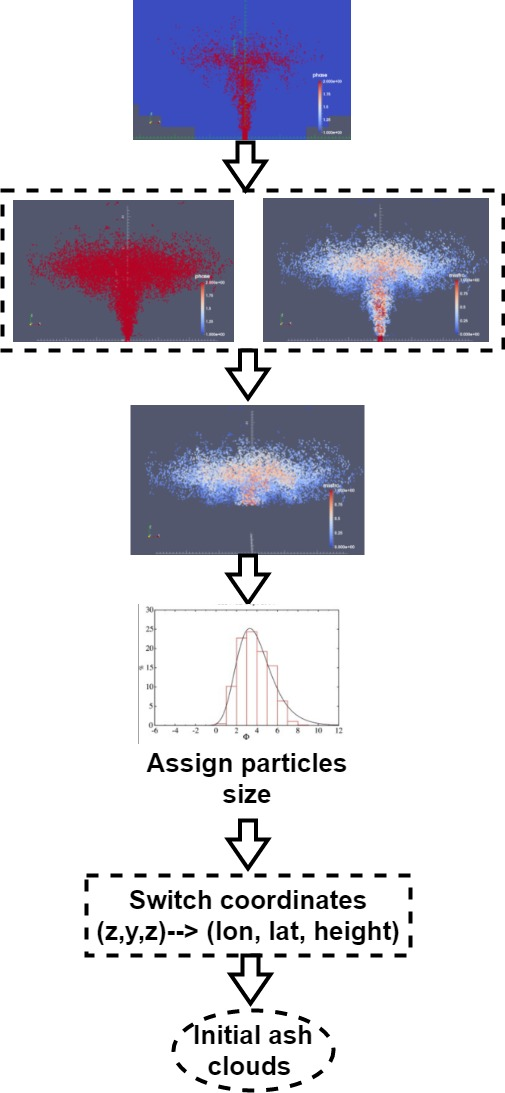
\includegraphics[width=0.43\textwidth]{Figures/Creat_initial_Ash}
\caption{Steps to create initial condition for Puff based on raw output of Plume-SPH \citep{cao2018plume}. First row: raw output of Plume-SPH. Blue particles are phase 1 (ambient air), red particles are phase 2 (erupted material). Second row: plume after removing SPH particles of phase 1. Picture at right is colored according to the mass fraction of erupted material. Third row: volcanic plume above the ``corner'' region after cutting off the lower portion. Fourth row: assign sizes to particles converting numerical discretization points into tracers. Fifth row: switch coordinates in local coordinate system into $(longitude, latitude, height)$}
\label{fig:create-initial-ash-plume-sph}
\end{figure}

\begin{figure}[!htb]
\centering
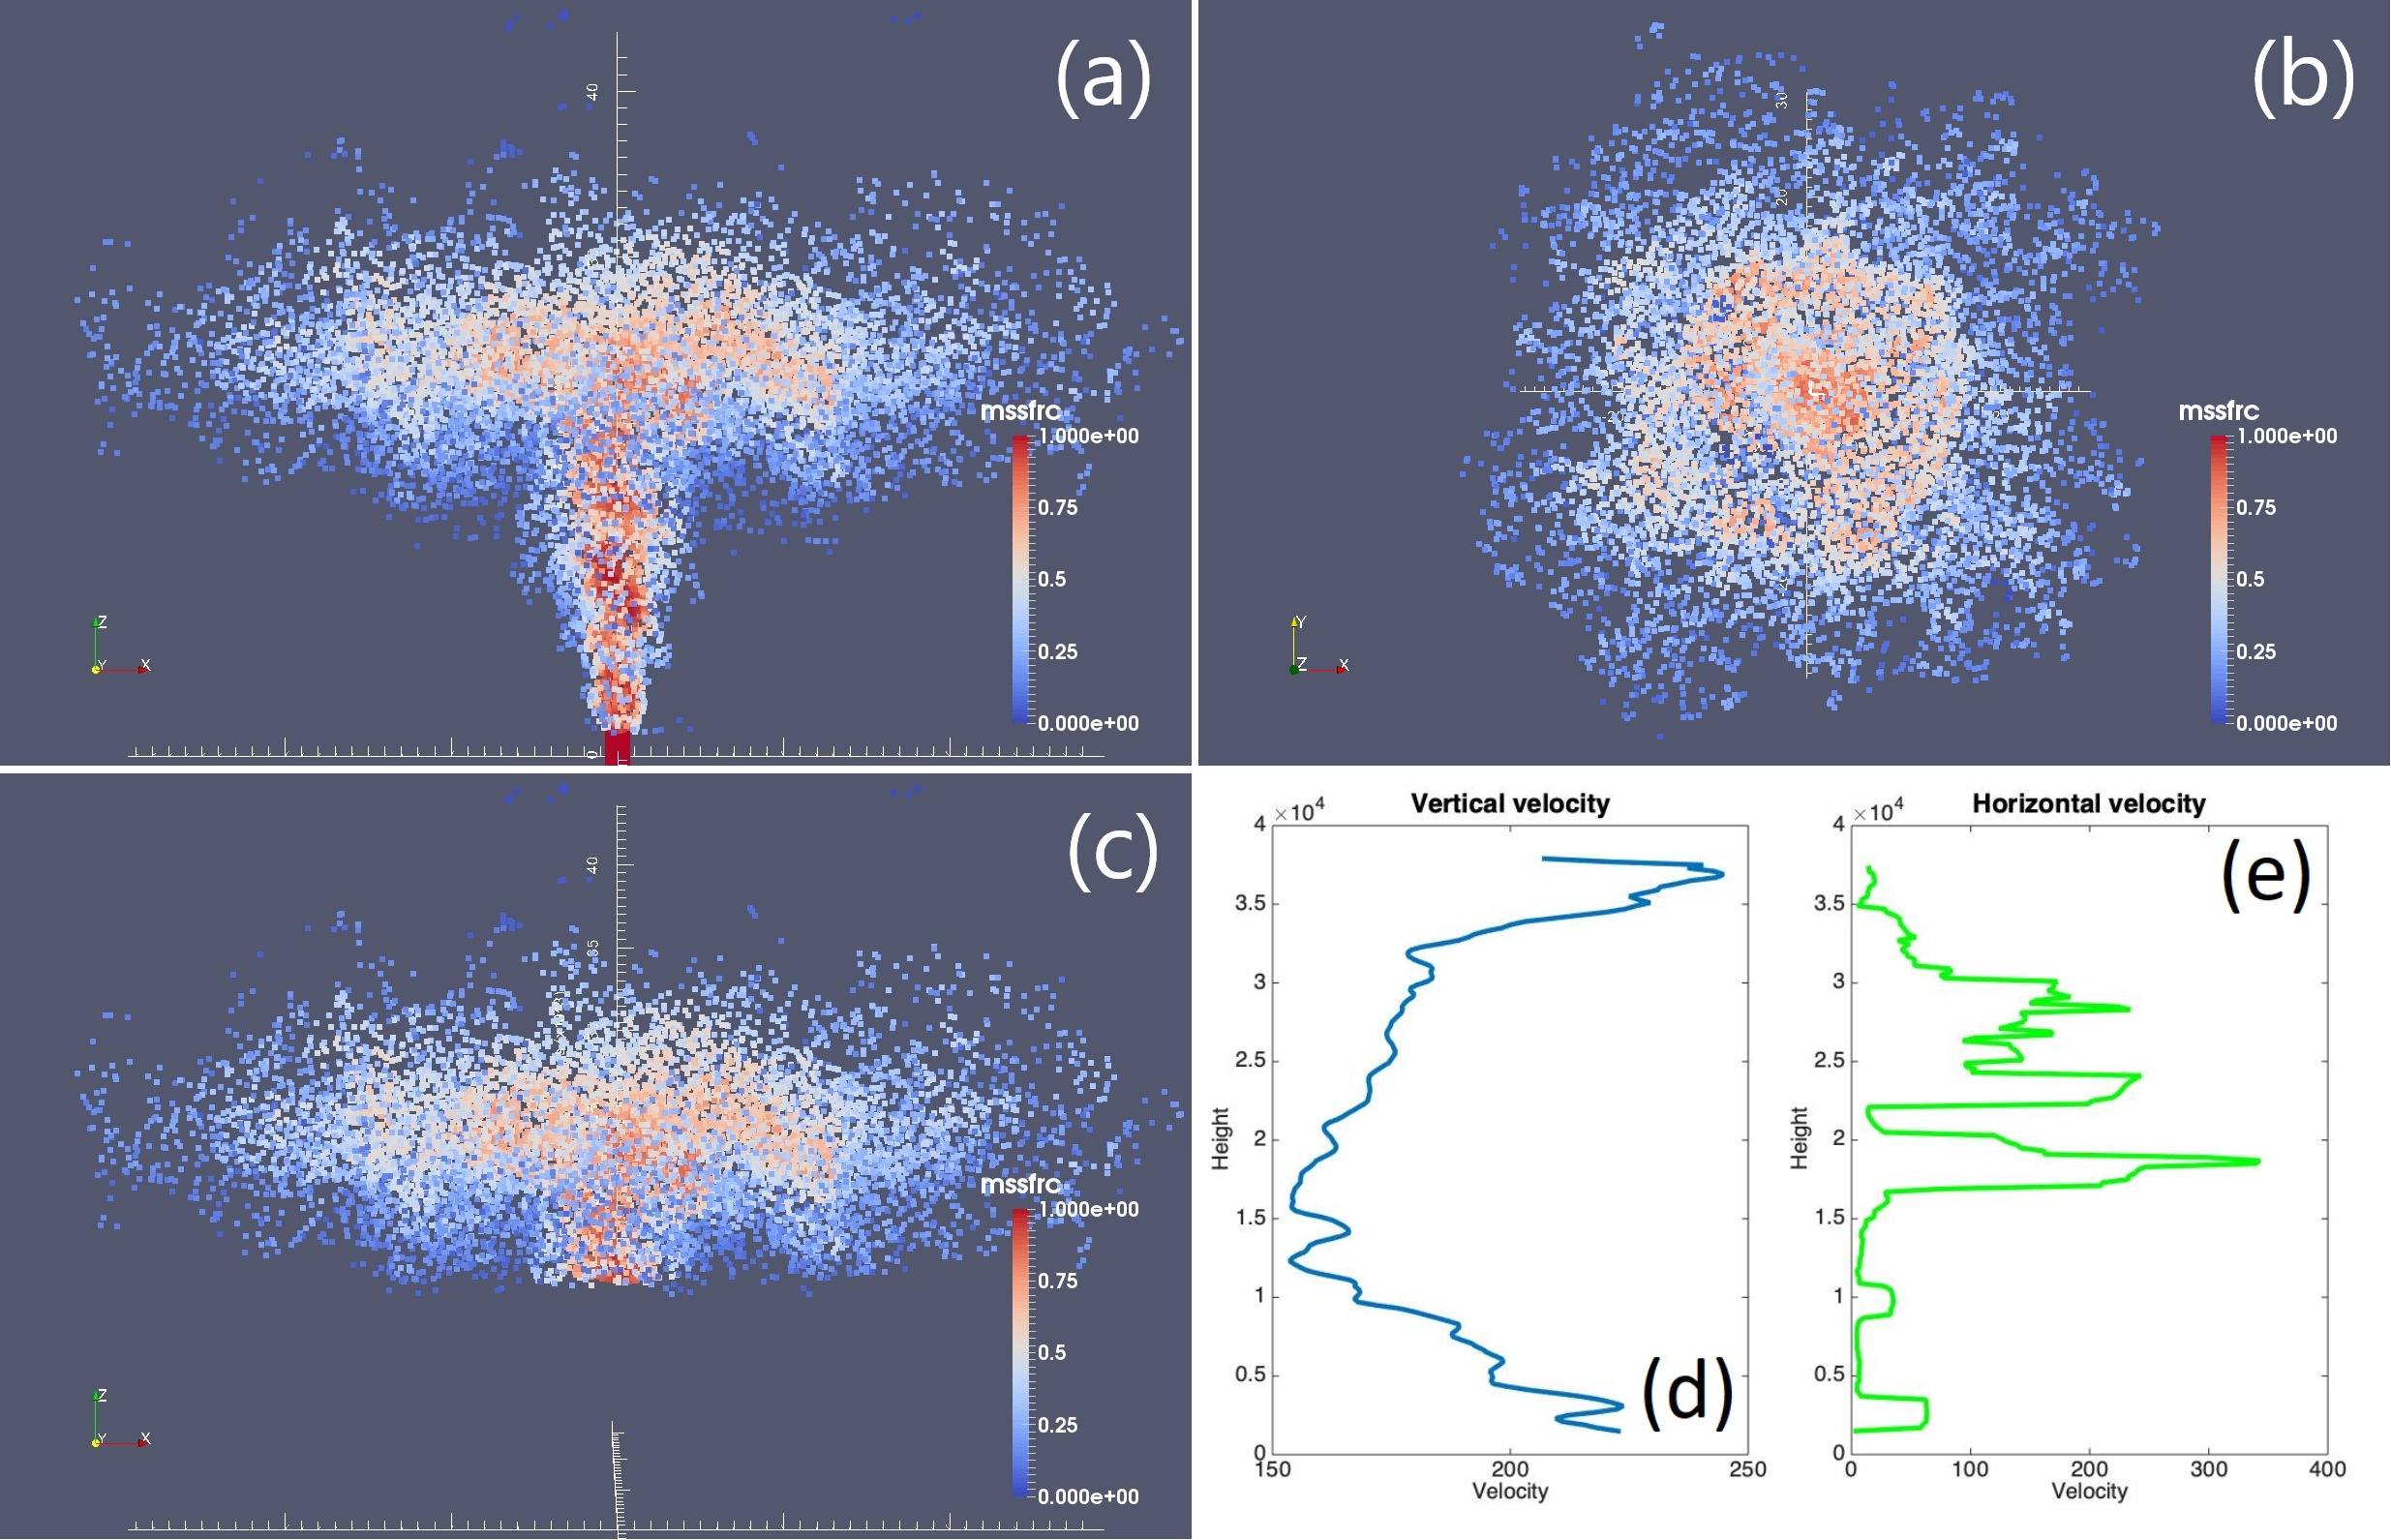
\includegraphics[width=1.0\textwidth]{Figures/Plume-SPH-Results}
\caption{Volcano plume from 3D plume model. All particles in the pictures are of  phase 2 (particle of phase 1 has been removed) at $600s$ after eruption, at which time, the plume has already reached the maximum height and started spreading radially. (a) is front view of the whole plume. (b) top view of the plume. (c) is front view of the initial ash cloud, which is essentially a portion of the whole plume with elevation higher than a given threshold (in this picture is $15000 m$). Particles are colored according to mass fraction of erupted material. Red represents high mass fraction while blue represents low mass fraction.}
\label{fig:Plume-SPH-Pinatubo-ash-cloud}
\end{figure}

\begin{figure}
\center
\includegraphics[width=0.90 \textwidth]{Figures/Restart-Puff}
\caption{Mimic successive eruption with intermittent pulsed releasing of ash particles. $t_I$ is the period of pulsing release. $t_I$ equals the physical time of 3D plume simulation.}
\label{fig:Restart-Puff}
\end{figure}

\begin{figure}[!htb]
\centering
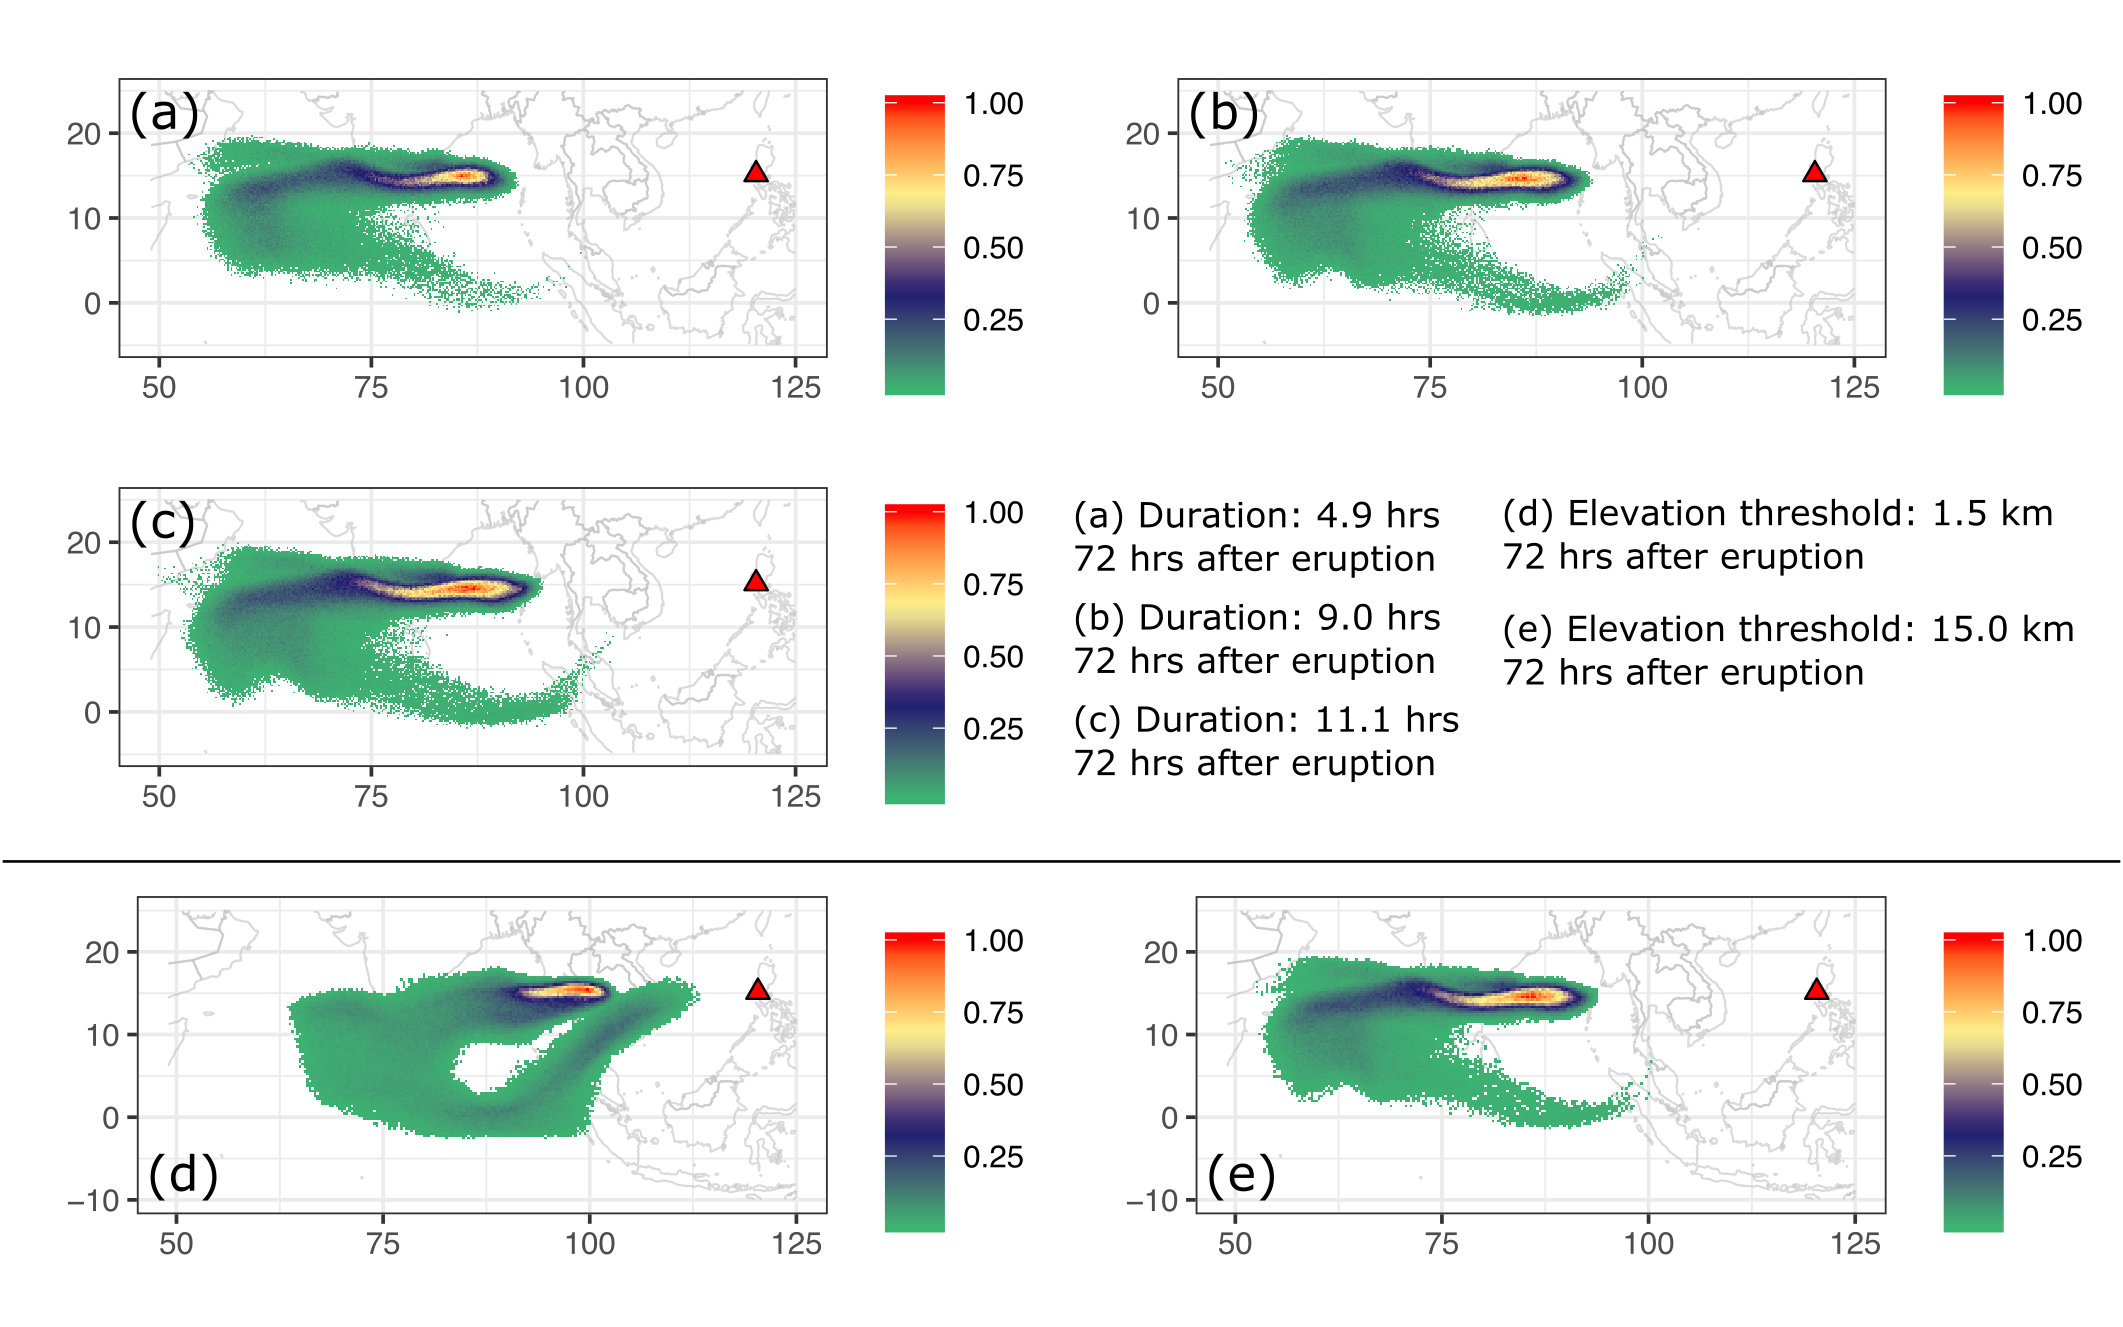
\includegraphics[width=0.99 \textwidth]{Figures/duration_cutoff}
\caption{Sensitivity of Puff simulation with respect to eruption durations and initial ash cloud cutoff heights .(a) to (c) are simulated ash distribution with different starting and ending time. They corresponding to eruption duration of 4.9 hours, 9 hours and 11.1 hours respectively. Starting and ending time for each case is in Table \ref{tab:Pinatubo-eruption-duration}. (d) and (e) are simulated ash distribution taking initial ash clouds obtained using different elevation thresholds ($1500 m$ and $15000$ m) from output of Plume-SPH. The starting and ending time are corresponding to 9 hours duration case in Table \ref{tab:Pinatubo-eruption-duration}. The contours correspond to ash concentration at 72 hours after eruption.}
\label{fig:Puff-sensitivity-duration-cutoff} 
\end{figure}

\begin{figure}[!htb]
\centering
\begin{minipage}{.75 \textwidth}
\centering
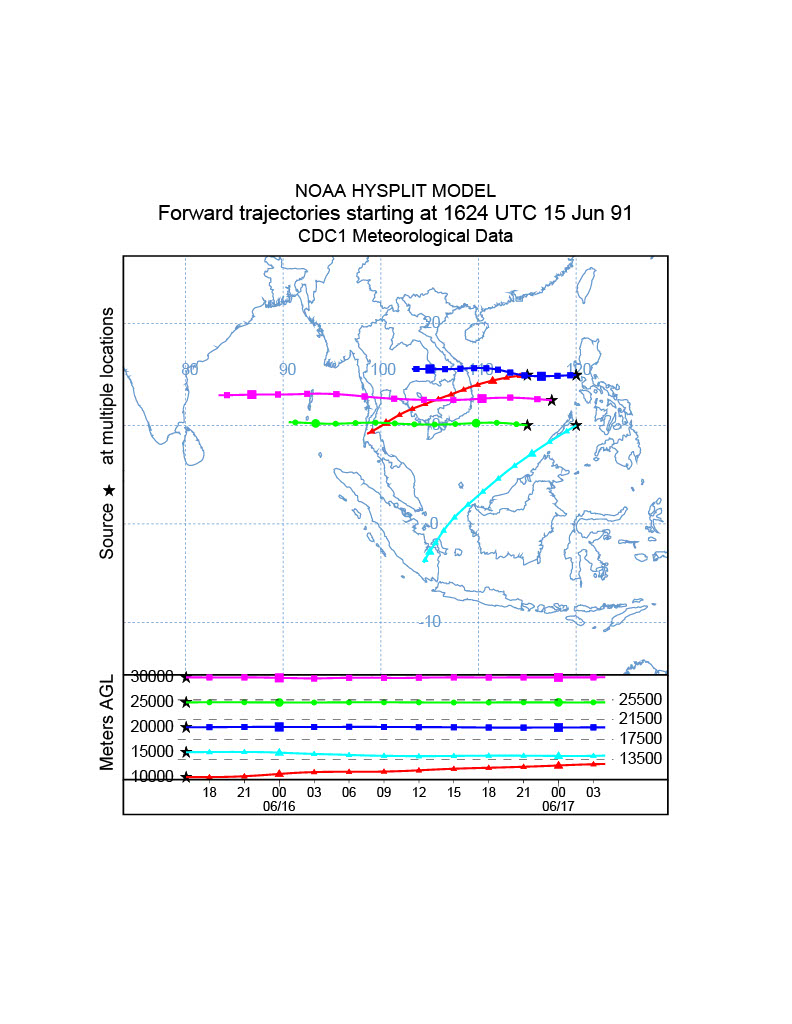
\includegraphics[width=0.99 \textwidth]{Figures/trajplot_test3_10_30K_ok}
\end{minipage}%
\caption{Trajectories of particles starting from different heights indicating the wind directions of different evaluations.}
\label{fig:hysplit-1624-utc}
\end{figure}

\begin{figure}[!htb]
\centering
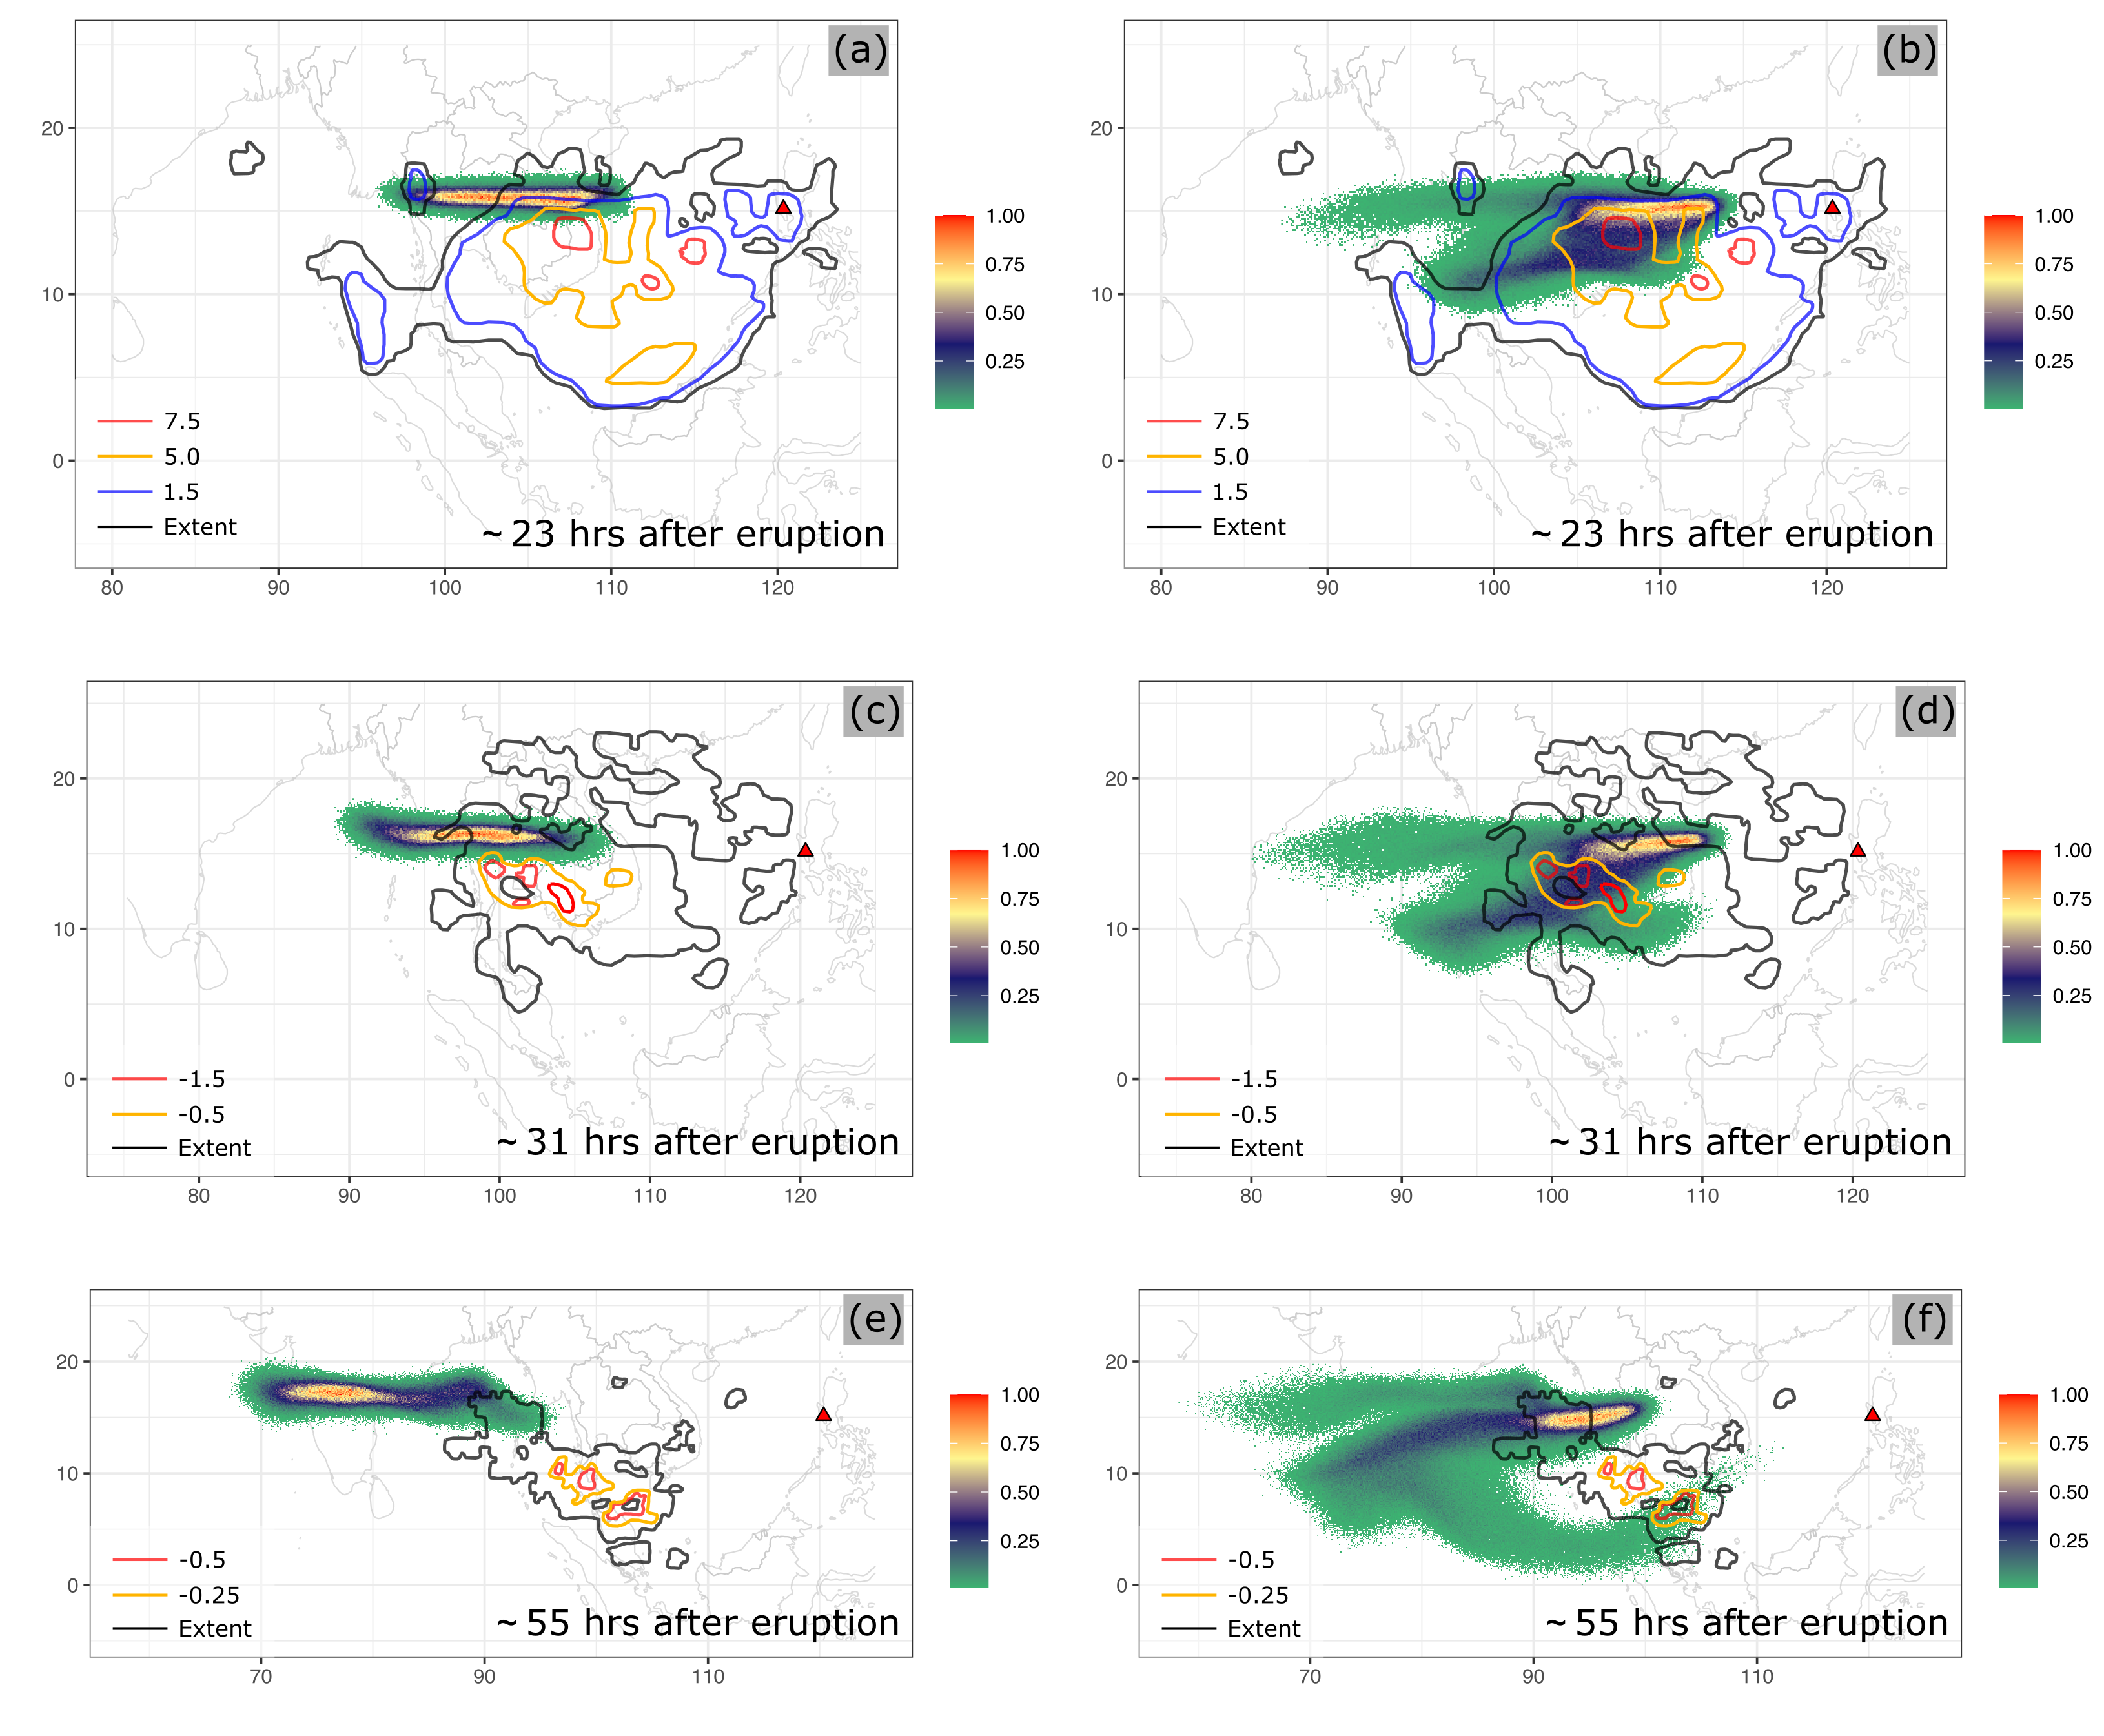
\includegraphics[width=0.99 \textwidth]{Figures/bent_plume}
\caption{Comparison between ``Semiempirical initial cloud + Puff" and ``Plume-SPH + Puff". Pictures to the left are: Puff simulation based on initial condition created according to semiempirical plume shape expression. Pictures to the right are Puff simulation based on initial condition generated by Plume-SPH. TOMS or AVHRR image of Pinatubo ash cloud are overlapped with the simulation results. Ash clouds at different hours after eruption are on different rows. From top to bottom, the images are corresponding to around 23 hours after eruption (UT 199106160341), 31 hours after eruption (UT 199106161141), 55 hours after eruption (UT 199106171141). The observation data on the first row are TOMS ash and ice map. The observation data on the second and third row are AVHRR BTD ash cloud map with atmospheric correction method applied \citep{guo2004particles}.}
\label{fig:Plume-SPH-Puff-ash-cloud}
\end{figure}

\begin{figure}[!htb]
\centering
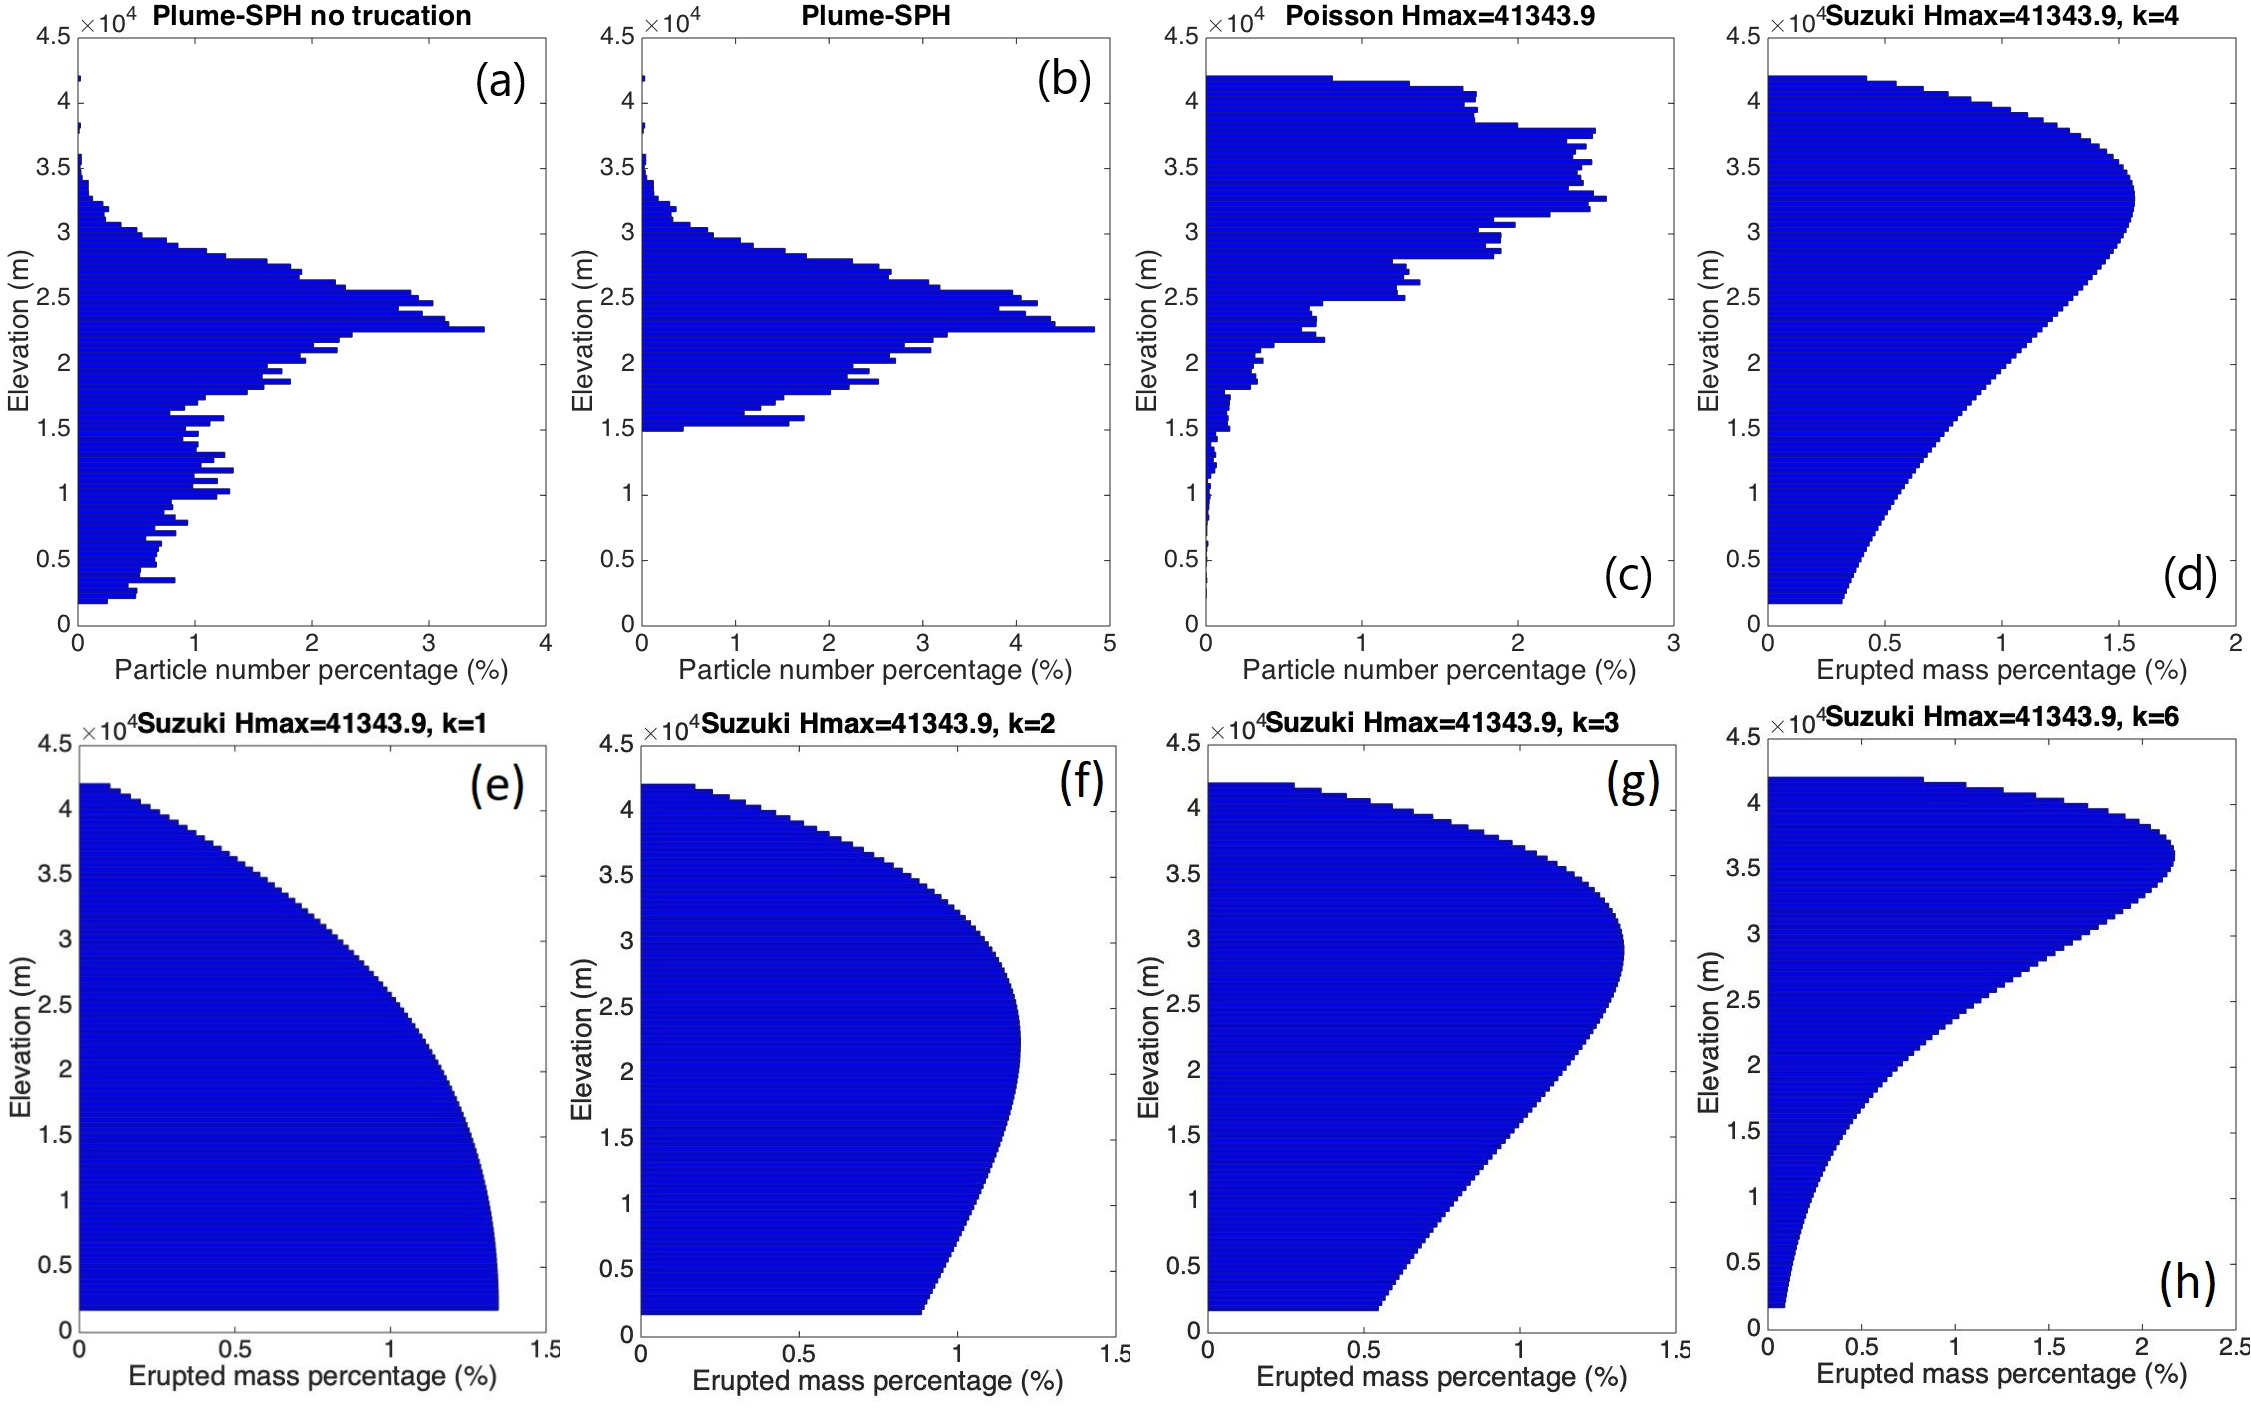
\includegraphics[width=1.0\textwidth]{Figures/particle_distribution_vertical_compare}
\caption{Particle distribution of initial ash cloud in vertical direction. (a) is corresponding to the initial ash cloud obtained from Plume-SPH output. (b) is corresponding to ash distribution of Plume-SPH output truncated by a elevation threshold of $15000 m$. (c) is for vertical ash distribution based on Poisson distribution with maximum height equals to $40000 m$. Another parameter, the vertical spread, in the expression of Poisson plume shape is $6662 m$. (d) is corresponding to Suzuki distribution with maximum height equals to $40000 m$. Another parameter in Suzuki distribution, the shape factor, is $4$. The $x$ axis is the percentage of particle numbers for Plume-SPH and Poisson. For Suzuki the $x$ axis is the mass percentage of erupted material.}
\label{fig:Particle-distribution-Plume-SPH-vs-semiempirical}
\end{figure}

\begin{figure}[!htb]
\centering
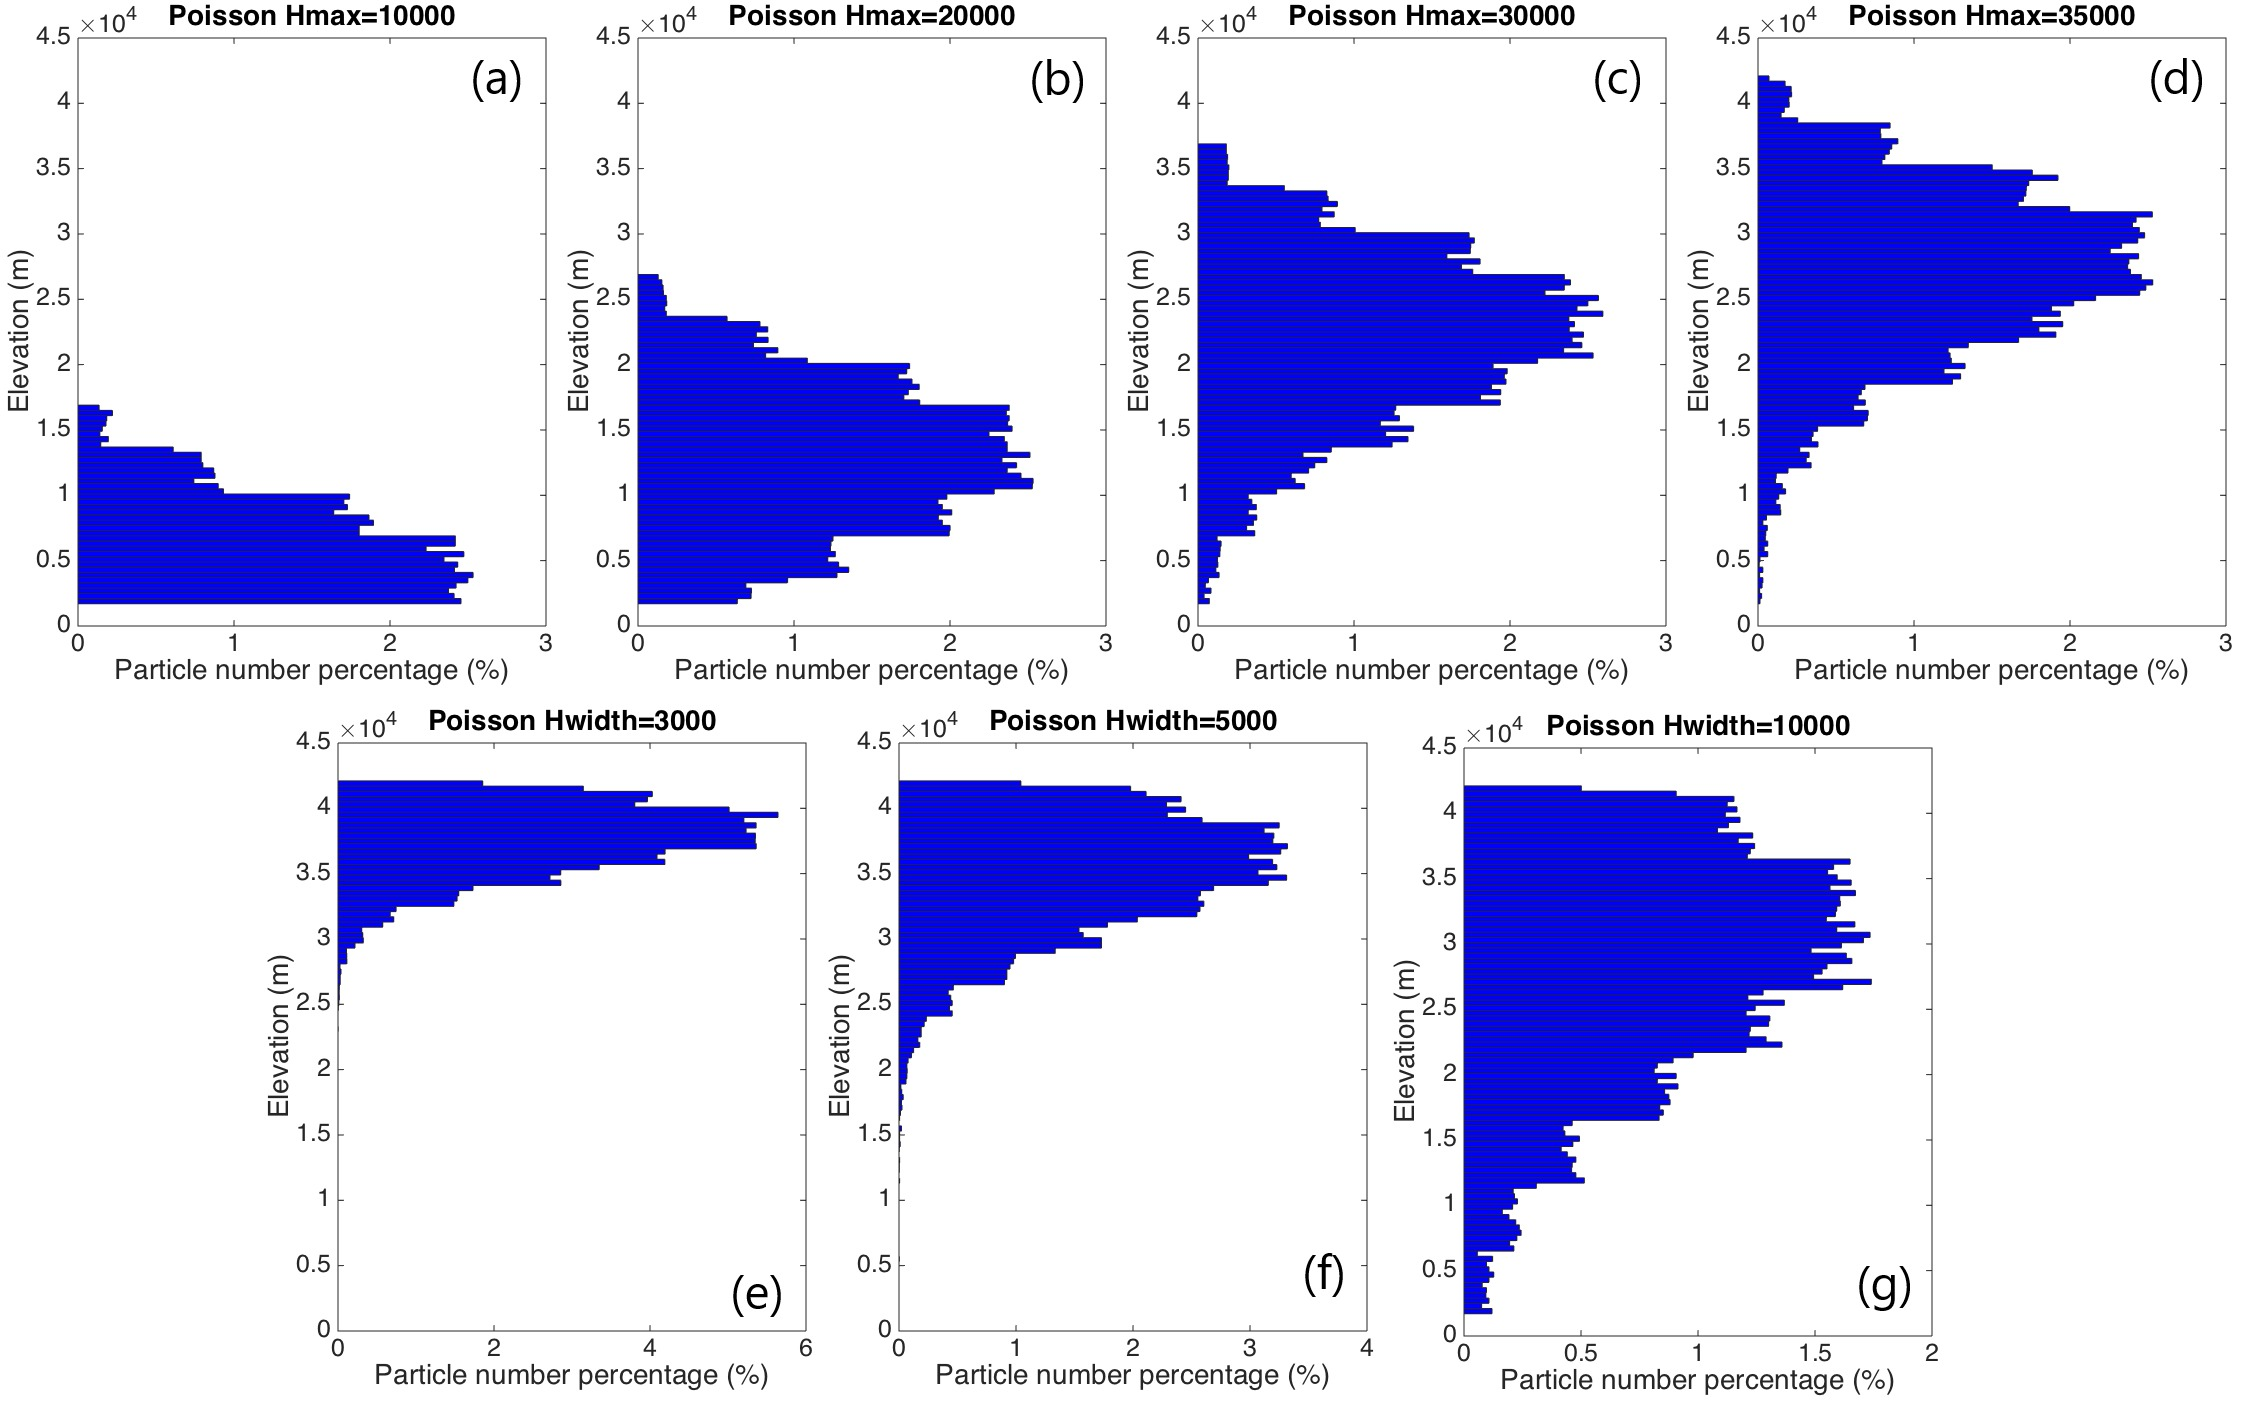
\includegraphics[width=1.0\textwidth]{Figures/particle_distribution_vertical_calibration}
\caption{Initial particle distribution in vertical direction based on Poisson plume shape. The first row varies maximum heights. (a) to (d) are corresponding to maximum height of $10000 m$, $20000 m$, $30000 m$, $35000 m$. Another parameter, the vertical spread, in the expression of Poisson plume shape is $6662 m$ for all four figures in the first row. The second row varies ``vertical spread". (e) to (g) are corresponding to vertical spread of $3km$, $5km$ and $10 km$. The maximum height in the expression of Poisson plume shape is $40000 m$ for all three figures. The $x$ axis is the percentage of particle numbers. See Fig. \ref{fig:Particle-distribution-Plume-SPH-vs-semiempirical} for vertical ash distribution of Plume-SPH output.}
\label{fig:Particle-distribution-Plume-calibrate-semiempirical}
\end{figure}

\begin{figure}[!htb]
\centering
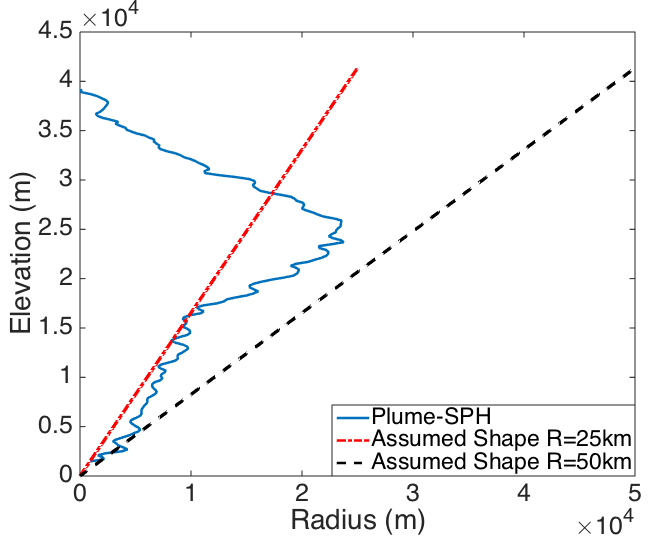
\includegraphics[width=0.50 \textwidth]{Figures/radius-Plume-SPH-And-Assumed}
\caption{Comparison between radius of initial ash clouds created by 3D plume model (Plume-SPH) and assumed initial ash cloud shape in Puff. The plume shape expression used in Puff defines an inverted cone whose actual shape changes when ``horizontal spread" takes different values. $R=25km$ is corresponding to ``horizontal spread" equals to $50km$. $R=50km$ is corresponding to ``horizontal spread" equals to $100km$}
\label{fig:radius-comparison}
\end{figure}

\begin{figure}[!htb]
\centering
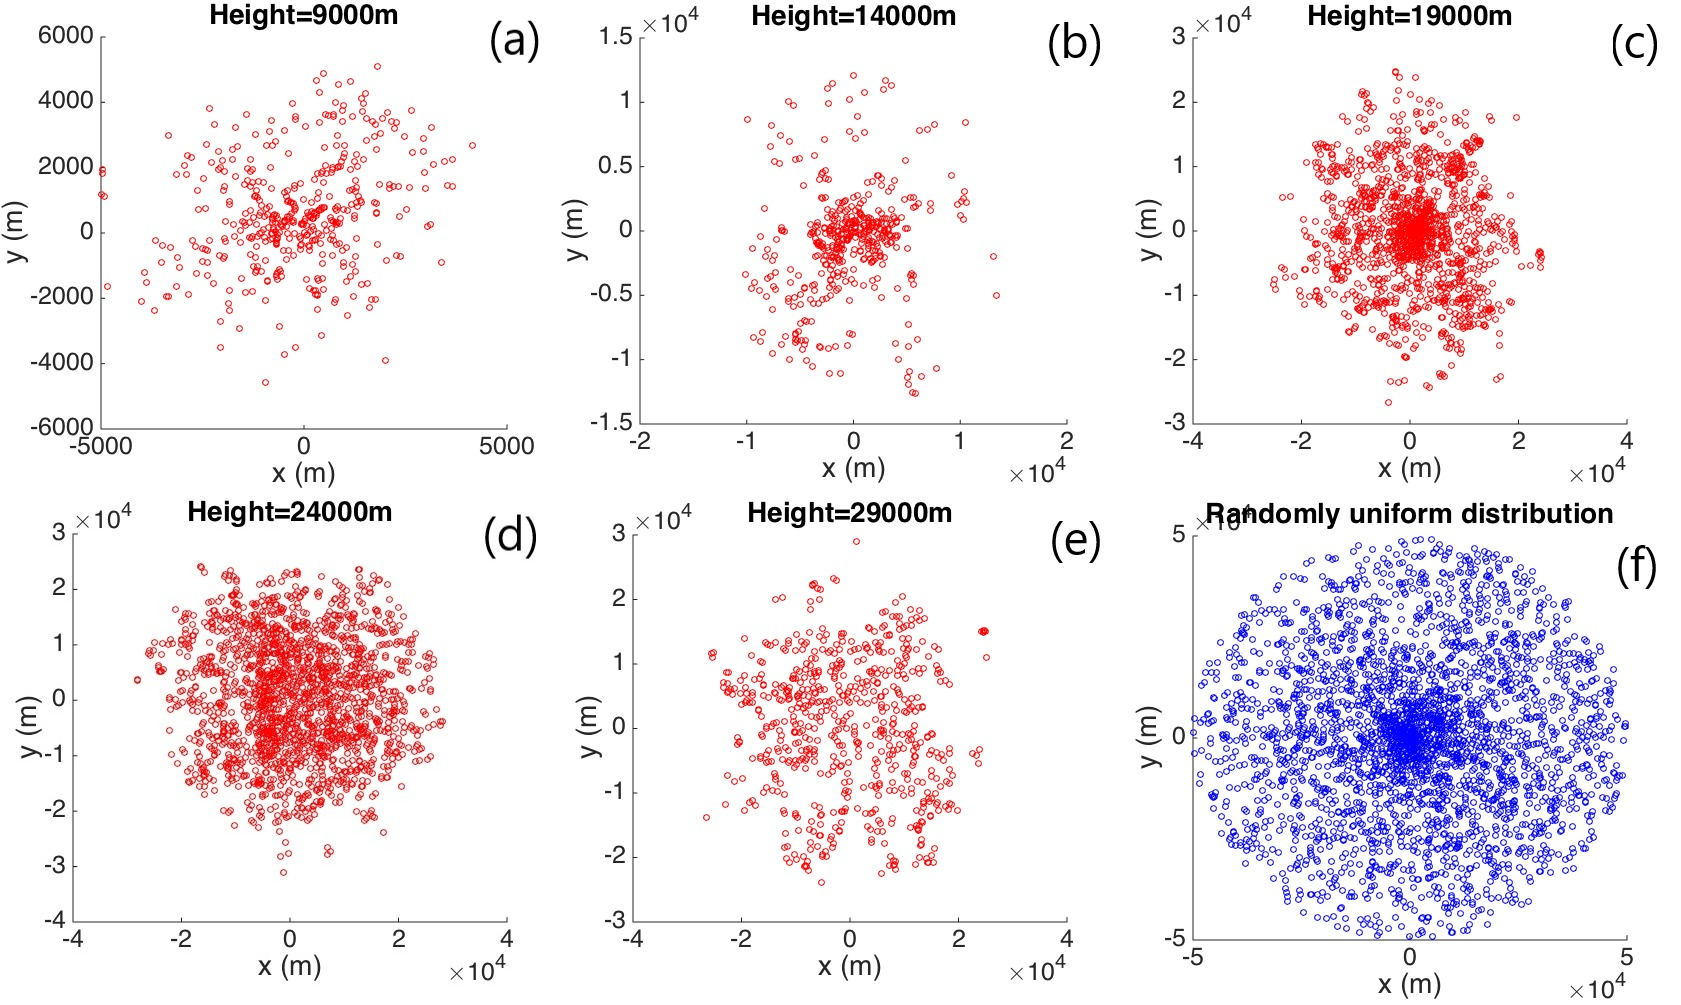
\includegraphics[width=1.0\textwidth]{Figures/particle_horizontal_distribution}
\caption{Horizontal distribution of ash particles (tracers) on a cross section of initial ash cloud. Puff assumes a randomly uniform distribution of ash particles within a circle, as shown by blue dots in (f). All other figures show the ash particle distribution of initial ash clouds created by Plume-SPH at different elevations.}
\label{fig:initial-cloud-horizontal}
\end{figure}


\begin{figure}[!htb]
\centering
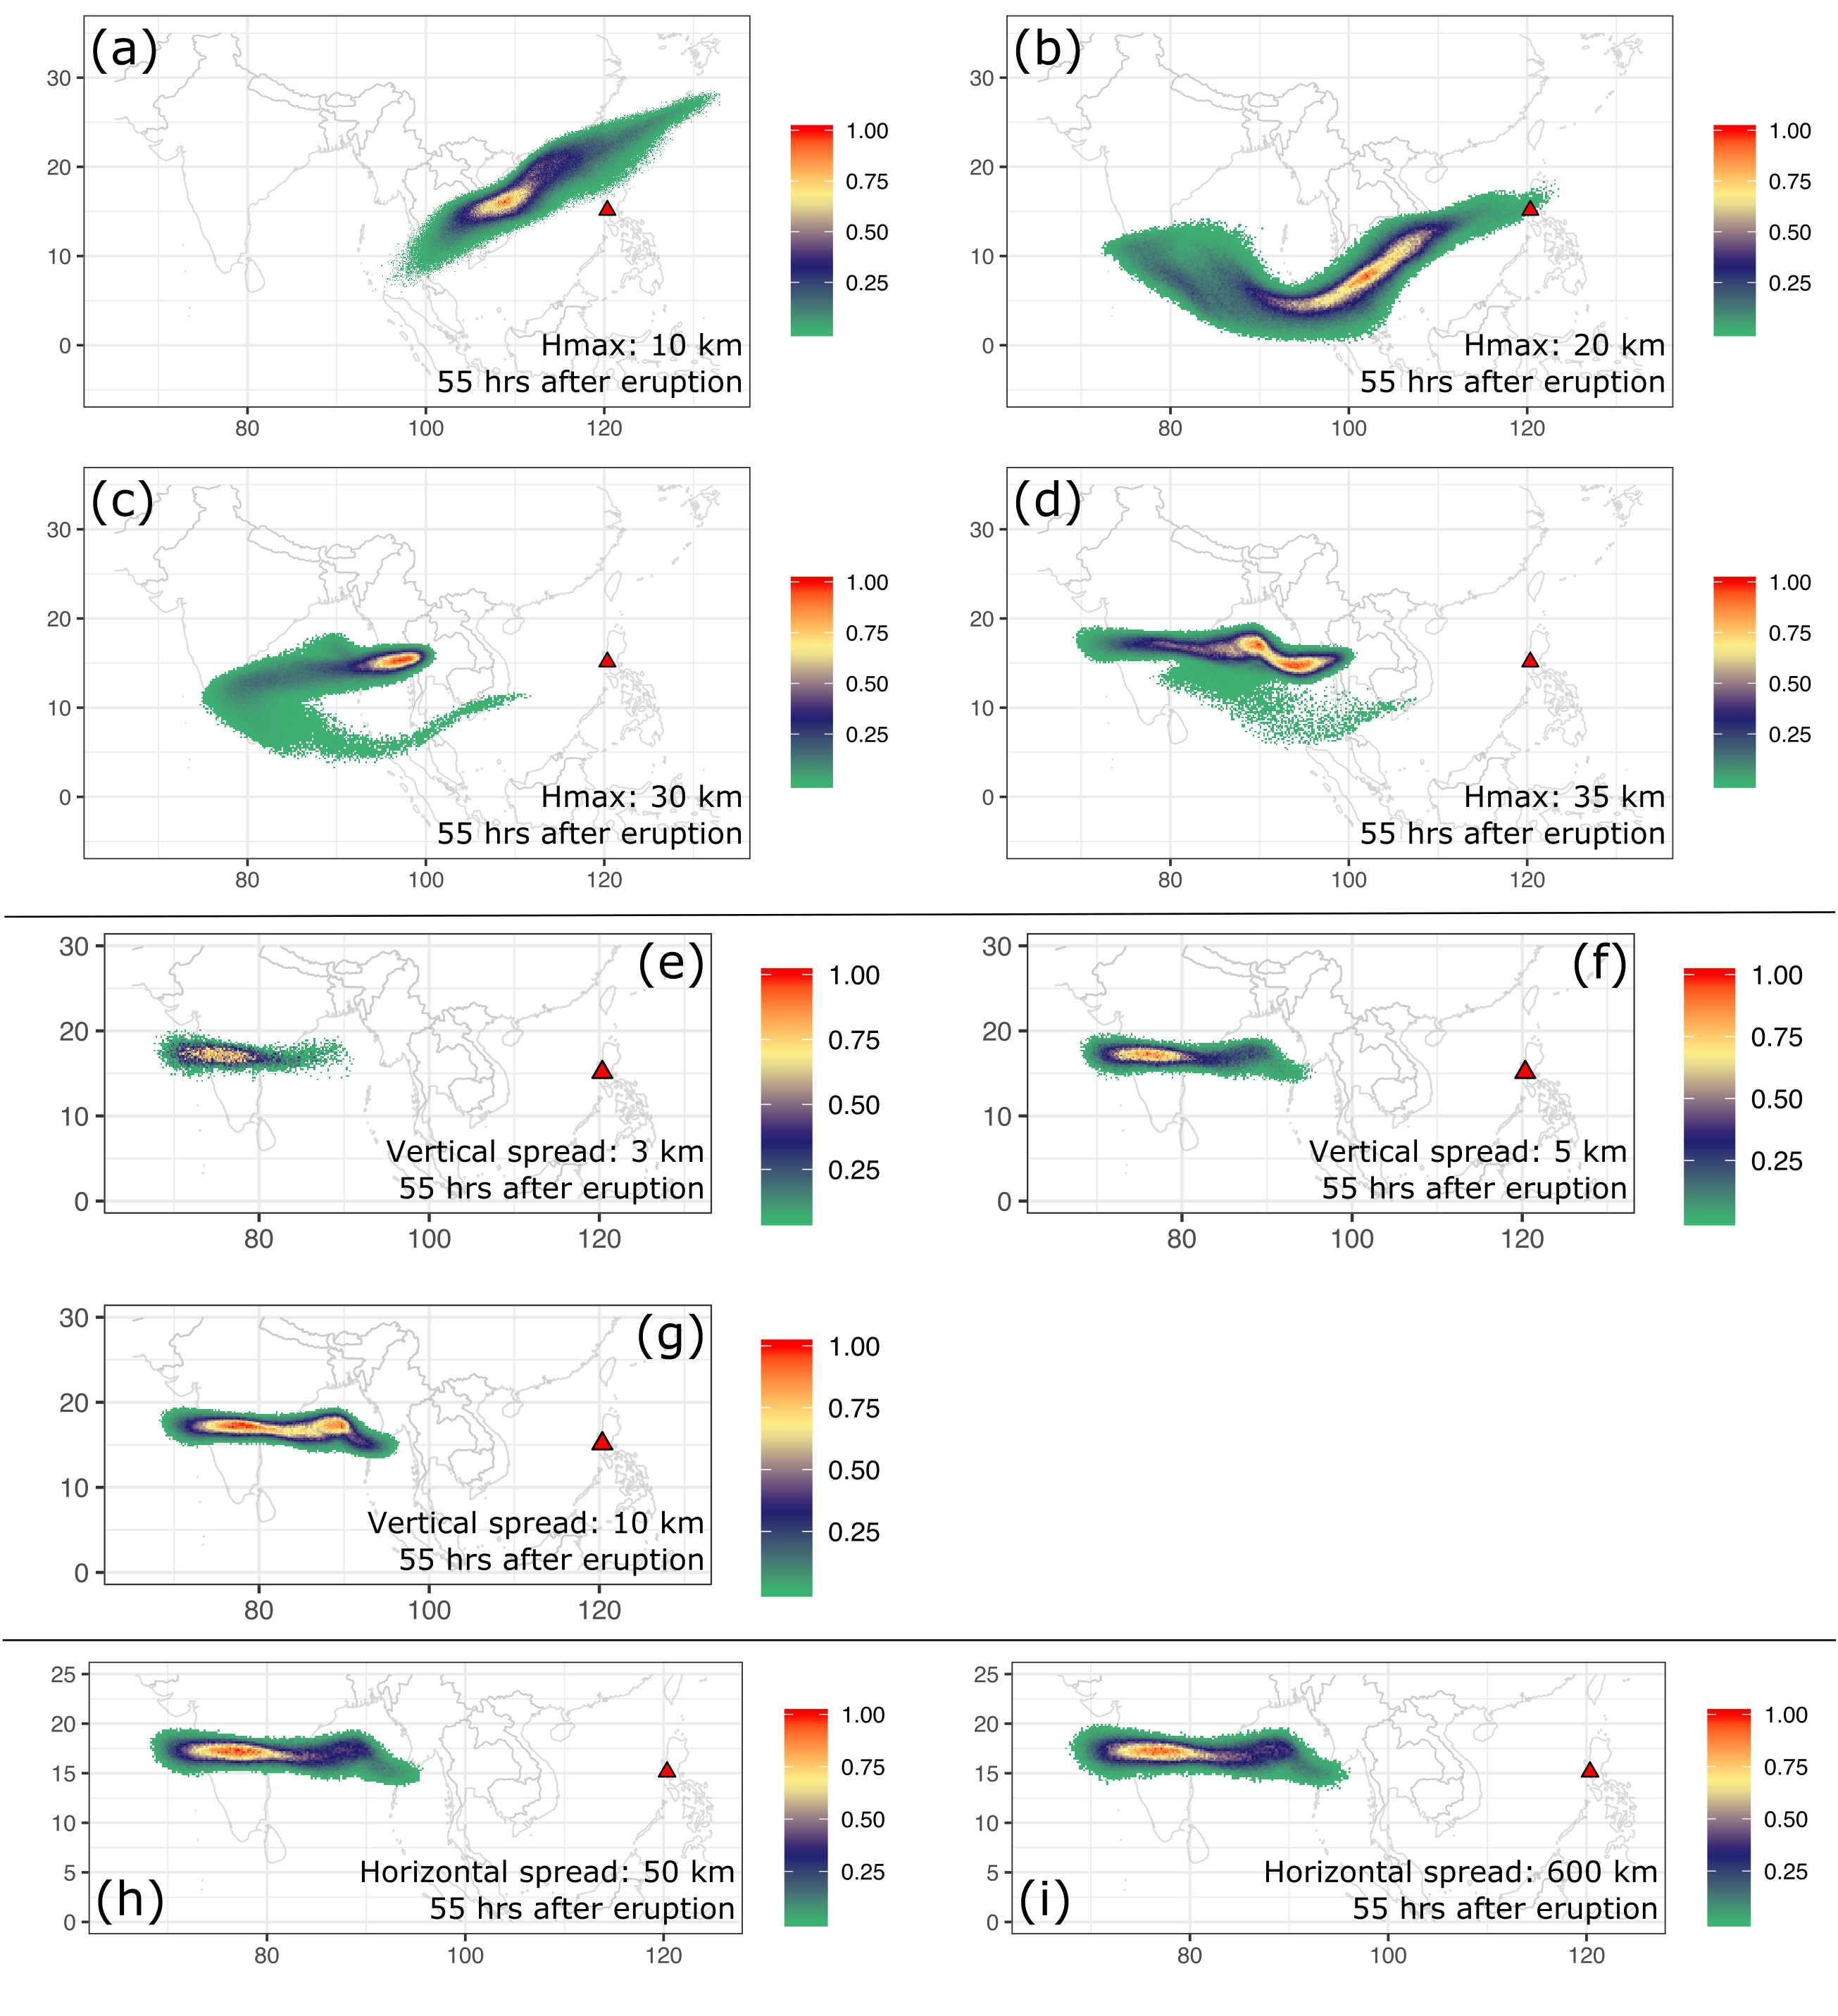
\includegraphics[width=0.99 \textwidth]{Figures/discussion}
\caption{Ash transport simulated by Puff using different initial ash clouds created according the empirical expressions. Initial ash cloud for (a) to (d)  are created according to Poisson distribution with maximum plume heights of $10km $, $20km$, $30km$ and $35km$ respectively.  Initial ash cloud for (e) to (g)  are created with vertical spread equals to $3km$, $5km$ and $10km$. respectively.  Initial ash cloud for (h) - (i)  are created with ``horizontal spread" equals to $50 km$ and $600km$ respectively. All images are for simulated ash transport around 55 hours after eruption (UT 199106171141). See the observed cloud image in Fig. \ref{fig:Plume-SPH-Puff-ash-cloud}.}
\label{fig:discussion-initial-ash}
\end{figure}

\begin{table}
\centering
\caption{Three different methods for creating initial conditions (initial ash clouds) for Puff simulation}		
	 \begin{tabular}{p{26.5mm}p{25.5mm}p{36.5mm}p{34.5mm}}
	 \hline
	 		 & No model & 1D model & 3D model \\
	 		 \hline 		
	 Maximum height & Calibration & Semiempirical & 1st principle \\
	 Average height & Calibration & Conservation laws (1D) & 1st principle \\
	 Vertical spread & Calibration & Semiempirical & 1st principle \\
	 Column radius & Calibration & Conservation laws (1D) & 1st principle \\
	 Plume shape & Semiempirical & Semiempirical & 1st principle \\
	 Tracers number & Free parameter & Free Parameter & Based on simulation\\
	 \hline
	 \end{tabular}
	 \label{tab:VATDs-source-term-determination}
\end{table}

\begin{table}[htp]
\centering
\caption{The starting and ending time (UT) for simulating the climactic phase of Pinatubo eruption on June 15 1991. Observed plume height \citep{holasek1996satellite} at different time are also listed in the table.}		
	 \begin{tabular}{p{35mm}p{20mm}p{20mm}p{20mm}p{20mm}}
	 \hline
Eruption duration & 4.9 hours & 9 hours & 10 hours & 11.1 hours \\
	 \hline
	 Start time & 0441 & 0441 & 0441 & 0334 \\
	 Height at start time & 37.5 km & 37.5 km & 37.5 km & 24.5 km \\
	
	 End time & 0934 & 1341 & 1441 & 1441 \\
	 	Height at end time & 35 km & 26.5 km & 22.5 & 22.5 km \\
	 \hline
	 \end{tabular}
	 \label{tab:Pinatubo-eruption-duration}
\end{table}


\begin{table}[htp]
	\centering
\caption{List of eruption condition and material properties for plume simulation}		
	 \begin{tabular}{lrr}
	 \hline
	 Parameters & Units & Plume \\
	 \hline
	 Vent velocity & $m\cdot s^{-1}$ & 275 \\
	 Vent gas mass fraction & & 0.05 \\
	 Vent Temperature & $K$ & 1053 \\
	 Vent height & $m$ & 1500 \\
	 Mass discharge rate & $kg\cdot s^{-1}$ & $1.5 \times 10^9$\\
	 	Specific heat of gas at constant volume & $J \cdot kg^{-1}\cdot K^{-1}$ & 717 \\
	 Specific heat of air at constant volume & $J \cdot kg^{-1}\cdot K^{-1}$ & 1340 \\
	 	Specific heat of solid & $J \cdot kg^{-1}\cdot K^{-1}$ & 1100 \\
	 	Specific heat of gas at constant pressure & $J \cdot kg^{-1}\cdot K^{-1}$ & 1000 \\
	 	Specific heat of air at constant pressure & $J \cdot kg^{-1}\cdot K^{-1}$ & 1810 \\
	 	Density of air at vent height & $kg \cdot m^{-3}$ & 1.104 \\
	 Pressure at vent height & $Pa$ & 84363.4 \\
	 \hline
	 \end{tabular}
	 \label{tab:input_parameters_plume_simulation}
\end{table}

\begin{table}[htp]
\centering
\caption{Parameters used in VATD simulation of the climactic phase of Pinatubo eruption on June 15 1991. The first six parameters are used by semiempirical expression to create an initial ash cloud. When creating an initial condition based on the Plume-SPH model, these parameters are extracted from output of Plume-SPH model.}
	 \begin{tabular}{lrrr}
	 \hline
	 Parameters & Unit & Semiempirical & Plume-SPH \\
	 \hline
	 Maximum Height ($H_{max}$) & $m$ & 40000 & - \\ %41800 \\
	 Horizontal Spread ($r_{max}$) & $km$ & 103.808 & -\\
	 Vertical Spread ($H_{width}$) & $km$ & 6.662 & - \\
	 Plume Shape & - & Poisson & - \\
	 Total Ash Particles & - & 1768500 & 1768500 \\
	 Elevation Threshold & $m$ & - & 15000 \\
	 Horizontal Diffusivity & $m^2/s$ &10000 & 10000\\
	 Vertical Diffusivity & $m^2/s$ & 10 & 10 \\
	 Grain Size Distribution & - & Gaussian & Gaussian \\
	 Mean of Grain Size (Radius) & $mm$ & $3.5 \times 10 ^-2$ & $3.5 \times 10 ^-2$ \\
	 Standard Deviation of Grain Size & - & 1.0 & 1.0 \\
	 	Start Time & UT & 0441 & 0441 \\
	 End time & UT & 1341 & 1341 \\
	 Simulation Duration & hour & 72 & 72 \\
	 \hline
	 \end{tabular}
	 \label{tab:input_parameter_Puff_simulation}
\end{table}
\end{document}
